\documentclass[aspectratio=169,10pt]{beamer}

\usepackage{beamerthemeLitSphere}
\usepackage{tabularx}
\usepackage{booktabs}
\usepackage{pifont}
\usepackage{colortbl}

\title{LitSphere}
\subtitle{A Collaborative Systematic Literature Review, Benchmark, and Research Synthesis Platform}
\author{Md Mostafa Kamal}
\institute{Department of Computer Science and Engineering \\ Jashore University of Science and Technology (JUST)}
\date{2026}

\begin{document}

% ==============================================================================
% SLIDE 1: Title Slide (White Theme matching Reference Design)
% ==============================================================================
\begin{frame}[plain]
\begin{tikzpicture}[remember picture,overlay]
  % Top Seal: Jashore University of Science and Technology
  \node[anchor=north] at ($(current page.north)+(0, -0.32cm)$) {%
    
\includegraphics[height=1.35cm,keepaspectratio]{figures/just_logo.png}%
  };

  % University and Department Header Text
  \node[anchor=north, align=center] at ($(current page.north)+(0, -1.48cm)$) {%
    {\fontsize{12.5pt}{15pt}\selectfont Jashore University of Science and Technology}\\[2.5pt]
    {\fontsize{10.5pt}{13pt}\selectfont Computer Science and Engineering}%
  };

  % Top Orange Divider Bar
  \draw[TitleOrange, line width=1.5pt] ($(current page.north west)+(1.0cm, -2.75cm)$) -- ($(current page.north east)+(-1.0cm, -2.75cm)$);

  % Project Title and Subtitle (Bold Rich Green)
  \node[anchor=center, align=center, text width=14.5cm] at ($(current page.north)+(0, -3.57cm)$) {%
    {\fontsize{17pt}{21pt}\selectfont\bfseries\color{TitleGreen} LitSphere}\\[4pt]
    {\fontsize{9.5pt}{13pt}\selectfont\bfseries\color{TitleGreen} A Collaborative Systematic Literature Review, Benchmark, and Research Synthesis Platform}%
  };

  % Bottom Orange Divider Bar
  \draw[TitleOrange, line width=1.5pt] ($(current page.north west)+(1.0cm, -4.40cm)$) -- ($(current page.north east)+(-1.0cm, -4.40cm)$);

  % Central Vertical Purple Divider Line
  \draw[DividerPurple, line width=4.0pt] ($(current page.center)+(0, -0.65cm)$) -- ($(current page.center)+(0, -3.20cm)$);

  % Presenter Information (Right-aligned to the left of the purple divider)
  \node[anchor=north east, align=right, text width=7.2cm] at ($(current page.center)+(-0.35cm, -0.68cm)$) {%
    {\fontsize{8.5pt}{12.5pt}\selectfont%
      \textbf{Presenter:}\\[2pt]
      Md Mostafa Kamal\\[2pt]
      Student Id: 200108\\[2pt]
      Dept. of Computer Science and Engineering(CSE)\\[2pt]
      Jashore University of Science and Technology%
    }%
  };

  % Supervisor Information (Left-aligned to the right of the purple divider)
  \node[anchor=north west, align=left, text width=7.2cm] at ($(current page.center)+(0.35cm, -0.60cm)$) {%
    {\fontsize{8.5pt}{12.5pt}\selectfont%
      \textbf{Supervisor:}\\[2pt]
      Dr. Mohammad Nowsin Amin Sheikh\\[2pt]
      Assistant Professor\\[2pt]
      B.Sc (Engg.), M.Sc (Engg.), PhD\\[2pt]
      Dept. of Computer Science and Engineering (CSE)\\[2pt]
      Jashore University of Science and Technology%
    }%
  };

  % Slide Counter (bottom right)
  \node[anchor=south east, font=\fontsize{8pt}{10pt}\selectfont] at ($(current page.south east)+(-0.6cm, 0.35cm)$) {%
    1/\inserttotalframenumber%
  };
\end{tikzpicture}
\end{frame}

% ==============================================================================
% SLIDE 2: Introduction & Research Motivation
% ==============================================================================
\begin{frame}{Introduction \& Research Motivation}
\vspace{-0.15cm}
\begin{columns}[T]
  \begin{column}{0.48\textwidth}
    \infoCard{6.8cm}{AccentAmber}{Challenge 01}{Scientific Literature Explosion}{%
      Over 1.5 million academic papers are published annually. Researchers face severe cognitive overload attempting to manually extract, index, and synthesize critical evidence across hundreds of PDF manuscripts.
    }\par\vspace{0.22cm}
    
    \infoCard{6.8cm}{AccentRed}{Challenge 02}{Fragmented Academic Toolchains}{%
      Reviewers are forced to juggle disconnected tools: Zotero for reference storage, Excel for data tables, and Word/Notepad for notes. This disjunction causes lost citations, data discrepancies, and workflow friction.
    }
  \end{column}
  
  \begin{column}{0.48\textwidth}
    \infoCard{6.8cm}{AccentTeal}{Limitation 03}{Absence of Coordinate Traceability}{%
      Conventional spreadsheets store extracted claims with zero link to source text. Verifying a recorded metric requires re-reading multi-page papers from scratch due to missing bounding-box coordinate anchors.
    }\par\vspace{0.22cm}
    
    \infoCard{6.8cm}{AccentGreen}{The Solution}{LitSphere Centralized Synthesis Platform}{%
      A unified, collaborative platform integrating split-screen PDF reading, coordinate-accurate claim anchoring, live synthesis matrix grids, and 1-click publication-ready LaTeX table generation.
    }
  \end{column}
\end{columns}
\end{frame}

% ==============================================================================
% SLIDE 3: Existing Systems & Limitations
% ==============================================================================
\begin{frame}{Existing Systems \& Limitations}
\vspace{-0.15cm}
\begin{columns}[T]
  \begin{column}{0.48\textwidth}
    \infoCard{6.8cm}{SubText}{Reference Managers}{Zotero, EndNote}{%
      \textbf{Strengths:} Reliable bibliographic indexing, citation metadata generation, and local PDF file storage.\\
      \textbf{Critical Gaps:} Incapable of structured variable extraction; zero comparative matrix synthesis; no PRISMA consensus screening.
    }\par\vspace{0.22cm}
    
    \infoCard{6.8cm}{SubText}{Manual Spreadsheets}{Microsoft Excel, Google Sheets}{%
      \textbf{Strengths:} Flexible rows and columns; universally accessible format.\\
      \textbf{Critical Gaps:} Completely detached from PDF documents; severe data entry error rates; zero coordinate-anchored text jump; high formatting overhead.
    }
  \end{column}
  
  \begin{column}{0.48\textwidth}
    \infoCard{6.8cm}{SubText}{Specialized SLR Tools}{Rayyan, Covidence}{%
      \textbf{Strengths:} Structured title/abstract screening for medical reviews.\\
      \textbf{Critical Gaps:} Prohibitive subscription paywalls; rigid clinical workflows; lack of interactive split-screen matrix extraction and benchmark clustering.
    }\par\vspace{0.22cm}
    
    \infoCard{6.8cm}{SubText}{Note-Taking Systems}{Obsidian, Notion, LiquidText}{%
      \textbf{Strengths:} Freeform markdown notes and visual document linking.\\
      \textbf{Critical Gaps:} Lack structured systematic review protocols; no multi-reviewer dual-blind voting; no automated LaTeX publication export.
    }
  \end{column}
\end{columns}
\end{frame}

% ==============================================================================
% SLIDE 4: LitSphere: Proposed System Architecture
% ==============================================================================
\begin{frame}{LitSphere: Proposed System Architecture}
\vspace{-0.15cm}
\centering
{\fontsize{8pt}{10pt}\selectfont\bfseries\color{SubText} CENTRALIZED COLLABORATIVE RESEARCH SYNTHESIS PLATFORM}\par\vspace{0.25cm}

\begin{columns}[T]
  \begin{column}{0.48\textwidth}
    {\fontsize{9.5pt}{11.5pt}\selectfont\bfseries\color{DarkText} Researcher Workspace: Dual-Pane Reviewer}\par\vspace{4pt}
    {\fontsize{7.5pt}{10pt}\selectfont\color{DarkText}
    \begin{itemize}
      \item \textbf{Split-Screen PDF Reader:} Synchronous in-browser PDF viewing without external software.
      \item \textbf{Coordinate BBox Anchoring:} Highlights are permanently bound to PDF page coordinates.
      \item \textbf{Direct Variable Extraction:} Populate dataset, model, metrics, and limitations side-by-side.
      \item \textbf{Search \& Tag Filter:} Instant filtering by keyword, publication year, and domain taxonomy.
    \end{itemize}}
  \end{column}

  \begin{column}{0.48\textwidth}
    {\fontsize{9.5pt}{11.5pt}\selectfont\bfseries\color{DarkText} Synthesis Lead: Master Matrix \& Analytics}\par\vspace{4pt}
    {\fontsize{7.5pt}{10pt}\selectfont\color{DarkText}
    \begin{itemize}
      \item \textbf{Interactive Master Matrix:} Unified comparative grid aggregating extracted variables across all papers.
      \item \textbf{Dynamic Clustering:} Automated thematic grouping by methodology, problem type, and results.
      \item \textbf{Dual-Blind PRISMA Engine:} Independent reviewer screening and Cohen's Kappa agreement check.
      \item \textbf{1-Click Academic Export:} Direct output to LaTeX \texttt{booktabs}, Excel (\texttt{.xlsx}), and BibTeX.
    \end{itemize}}
  \end{column}
\end{columns}

\vspace{0.45cm}
\rule{14.2cm}{0.4pt}\par\vspace{0.12cm}
{\centering\fontsize{7.5pt}{9.5pt}\selectfont\color{DarkText}
\textbf{Core Impact:} Eliminates the 80\% administrative friction between reading academic literature and synthesizing publishable survey articles.\par}
\end{frame}

% ==============================================================================
% SLIDE 5: Feature Comparison Matrix
% ==============================================================================
\begin{frame}{Feature Comparison: LitSphere vs.\ Existing Tools}
\vspace{-0.2cm}
\centering
\fontsize{7.2pt}{10pt}\selectfont
\begin{tabularx}{14.5cm}{lcccc}
\toprule
\textbf{Feature Dimension} & 
\textbf{Zotero} & 
\textbf{MS Excel / Sheets} & 
\textbf{Rayyan / Covidence} & 
\textbf{LitSphere (Proposed)} \\
\midrule
In-Browser PDF Annotation & \ding{51} (Basic) & \ding{55} & \ding{55} & \textbf{\color{AccentGreen}\ding{51} (Dual-Pane)} \\
Coordinate-Anchored Claims & \ding{55} & \ding{55} & \ding{55} & \textbf{\color{AccentGreen}\ding{51} (Exact BBox)} \\
Master Synthesis Matrix Grid & \ding{55} & \ding{51} (Manual) & \ding{55} & \textbf{\color{AccentGreen}\ding{51} (Real-Time)} \\
Thematic Clustering & \ding{55} & \ding{55} & \ding{55} & \textbf{\color{AccentGreen}\ding{51} (Taxonomy)} \\
Dual-Blind PRISMA Screening & \ding{55} & \ding{55} & \ding{51} (Paid) & \textbf{\color{AccentGreen}\ding{51} (Built-in)} \\
One-Click LaTeX \texttt{booktabs} Export & \ding{55} & \ding{55} & \ding{55} & \textbf{\color{AccentGreen}\ding{51} (Native)} \\
Local-First SQLite WAL Storage & \ding{51} (Proprietary) & \ding{55} & \ding{55} (Cloud-only) & \textbf{\color{AccentGreen}\ding{51} (Open ACID)} \\
Zero-Framework Sub-15ms Latency & \ding{55} & \ding{55} & \ding{55} & \textbf{\color{AccentGreen}\ding{51} (Optimized)} \\
\bottomrule
\end{tabularx}

\vspace{0.4cm}
\begin{columns}[T]
  \begin{column}{0.31\textwidth}
    \infoCard{4.3cm}{AccentGreen}{Verifiability}{100\% Traceability}{%
      Every extracted claim jumps directly to its original sentence in the PDF.
    }
  \end{column}
  \begin{column}{0.31\textwidth}
    \infoCard{4.3cm}{SubText}{Standards}{PRISMA Compliance}{%
      Structured screening, consensus voting, and automated exclusion reporting.
    }
  \end{column}
  \begin{column}{0.31\textwidth}
    \infoCard{4.3cm}{AccentAmber}{Efficiency}{Publication-Ready}{%
      Direct generation of publication-grade LaTeX tables and BibTeX citation keys.
    }
  \end{column}
\end{columns}
\end{frame}

% ==============================================================================
% SLIDE 6: Advanced Features: Part 1
% ==============================================================================
\begin{frame}{Advanced Features: LitSphere Advantage (Part 1)}
\vspace{-0.15cm}
\begin{columns}[T]
  \begin{column}{0.31\textwidth}
    {\fontsize{6.8pt}{8.5pt}\selectfont\bfseries\color{SubText} FEATURE MODULE 01}\par\vspace{2pt}
    {\fontsize{9.5pt}{11.5pt}\selectfont\bfseries\color{DarkText} Split-Screen Dual-Pane Reviewer}\par\vspace{4pt}
    {\fontsize{7.2pt}{9.2pt}\selectfont\color{DarkText}
    \begin{itemize}
      \item Synchronous side-by-side layout: PDF reader docked alongside data extraction form.
      \item Eliminates disruptive Alt-Tab switching between viewer and external spreadsheets.
      \item Native PDF.js rendering with continuous vertical scrolling, zoom, and page jump.
    \end{itemize}}
  \end{column}

  \begin{column}{0.31\textwidth}
    {\fontsize{6.8pt}{8.5pt}\selectfont\bfseries\color{SubText} FEATURE MODULE 02}\par\vspace{2pt}
    {\fontsize{9.5pt}{11.5pt}\selectfont\bfseries\color{DarkText} Coordinate-Accurate Text Highlighting}\par\vspace{4pt}
    {\fontsize{7.2pt}{9.2pt}\selectfont\color{DarkText}
    \begin{itemize}
      \item Bounding box coordinates recorded in normalized $[x, y, w, h]$ geometry.
      \item Highlighting survives zoom, scaling, and responsive viewport adjustments.
      \item Clicking an extracted matrix metric instantly navigates to the exact sentence.
    \end{itemize}}
  \end{column}

  \begin{column}{0.31\textwidth}
    {\fontsize{6.8pt}{8.5pt}\selectfont\bfseries\color{SubText} FEATURE MODULE 03}\par\vspace{2pt}
    {\fontsize{9.5pt}{11.5pt}\selectfont\bfseries\color{DarkText} Master Synthesis Matrix Grid}\par\vspace{4pt}
    {\fontsize{7.2pt}{9.2pt}\selectfont\color{DarkText}
    \begin{itemize}
      \item Real-time multi-dimensional comparison table across all ingested papers.
      \item Inline editing with instant database persistence and audit trails.
      \item Dynamic filtering by publication year, taxonomy tags, and performance metrics.
    \end{itemize}}
  \end{column}
\end{columns}

\vspace{0.45cm}
\rule{14.2cm}{0.4pt}\par\vspace{0.12cm}
{\fontsize{7.2pt}{9pt}\selectfont\color{DarkText}
\textbf{Engineering Significance:} These three interconnected capabilities create a closed-loop verification cycle, guaranteeing that every scientific claim in the synthesis matrix is verifiable in under 2 seconds.}
\end{frame}

% ==============================================================================
% SLIDE 7: Advanced Features: Part 2
% ==============================================================================
\begin{frame}{Advanced Features: LitSphere Advantage (Part 2)}
\vspace{-0.15cm}
\begin{columns}[T]
  \begin{column}{0.31\textwidth}
    {\fontsize{6.8pt}{8.5pt}\selectfont\bfseries\color{SubText} FEATURE MODULE 04}\par\vspace{2pt}
    {\fontsize{9.5pt}{11.5pt}\selectfont\bfseries\color{DarkText} Dual-Blind PRISMA Screening}\par\vspace{4pt}
    {\fontsize{7.2pt}{9.2pt}\selectfont\color{DarkText}
    \begin{itemize}
      \item Independent voting protocol (Include / Exclude / Maybe) for peer reviewers.
      \item Automated calculation of Cohen's Kappa ($\kappa$) inter-rater agreement score.
      \item Arbitration interface for lead supervisors to resolve inclusion conflicts.
    \end{itemize}}
  \end{column}

  \begin{column}{0.31\textwidth}
    {\fontsize{6.8pt}{8.5pt}\selectfont\bfseries\color{SubText} FEATURE MODULE 05}\par\vspace{2pt}
    {\fontsize{9.5pt}{11.5pt}\selectfont\bfseries\color{DarkText} Zero-Framework High Performance}\par\vspace{4pt}
    {\fontsize{7.2pt}{9.2pt}\selectfont\color{DarkText}
    \begin{itemize}
      \item Built entirely using Vanilla ES6 JavaScript without bloated runtime frameworks.
      \item Sub-15ms client interaction latency and ultra-fast DOM redraw speeds.
      \item SQLite WAL mode enables concurrent reader execution with zero locking stalls.
    \end{itemize}}
  \end{column}

  \begin{column}{0.31\textwidth}
    {\fontsize{6.8pt}{8.5pt}\selectfont\bfseries\color{SubText} FEATURE MODULE 06}\par\vspace{2pt}
    {\fontsize{9.5pt}{11.5pt}\selectfont\bfseries\color{DarkText} 1-Click Academic Export Engine}\par\vspace{4pt}
    {\fontsize{7.2pt}{9.2pt}\selectfont\color{DarkText}
    \begin{itemize}
      \item Direct generation of IEEE/ACM compliant LaTeX \texttt{booktabs} code tables.
      \item Formatted Excel export (\texttt{.xlsx}) for statistical meta-analysis.
      \item Automatic BibTeX synchronization with sanitized citation keys and DOIs.
    \end{itemize}}
  \end{column}
\end{columns}

\vspace{0.45cm}
\rule{14.2cm}{0.4pt}\par\vspace{0.12cm}
{\fontsize{7.2pt}{9pt}\selectfont\color{DarkText}
\textbf{Research Rigor:} Conforms to international PRISMA (Preferred Reporting Items for Systematic Reviews and Meta-Analyses) guidelines, ensuring standard-compliant literature reviews.}
\end{frame}

% ==============================================================================
% SLIDE 8: System Architecture & Technology Stack
% ==============================================================================
\begin{frame}{System Architecture \& Technology Stack}
\vspace{-0.15cm}
\begin{columns}[T]
  \begin{column}{0.31\textwidth}
    {\fontsize{7pt}{8.5pt}\selectfont\bfseries\color{SubText} FRONTEND LAYER}\par\vspace{2pt}
    {\fontsize{9.5pt}{11.5pt}\selectfont\bfseries\color{DarkText} Native Web Architecture}\par\vspace{4pt}
    {\fontsize{7.2pt}{9.2pt}\selectfont\color{DarkText}
    \begin{itemize}
      \item \textbf{HTML5 \& CSS3:} Modular design tokens, light theme, CSS grid and flexbox.
      \item \textbf{Vanilla ES6 JS:} High performance, zero dependency bundle overhead.
      \item \textbf{PDF.js Library:} Mozilla client-side PDF rendering engine.
      \item \textbf{Canvas Overlay:} Coordinate highlight layer with precise BBox geometry.
    \end{itemize}}
  \end{column}

  \begin{column}{0.31\textwidth}
    {\fontsize{7pt}{8.5pt}\selectfont\bfseries\color{SubText} BACKEND LAYER}\par\vspace{2pt}
    {\fontsize{9.5pt}{11.5pt}\selectfont\bfseries\color{DarkText} Node.js REST API Service}\par\vspace{4pt}
    {\fontsize{7.2pt}{9.2pt}\selectfont\color{DarkText}
    \begin{itemize}
      \item \textbf{Node.js \& Express:} Non-blocking asynchronous event-driven I/O.
      \item \textbf{Multer Engine:} Streaming multipart PDF ingestion and validation.
      \item \textbf{JWT Security:} Stateless authorization with bcrypt hash encryption.
      \item \textbf{Export Pipeline:} Programmatic LaTeX table and XLSX synthesis.
    \end{itemize}}
  \end{column}

  \begin{column}{0.31\textwidth}
    {\fontsize{7pt}{8.5pt}\selectfont\bfseries\color{SubText} PERSISTENCE LAYER}\par\vspace{2pt}
    {\fontsize{9.5pt}{11.5pt}\selectfont\bfseries\color{DarkText} SQLite 3 Database Engine}\par\vspace{4pt}
    {\fontsize{7.2pt}{9.2pt}\selectfont\color{DarkText}
    \begin{itemize}
      \item \textbf{SQLite 3 Engine:} Embedded, zero-configuration relational database.
      \item \textbf{WAL Mode:} Write-Ahead Logging for high-throughput concurrency.
      \item \textbf{ACID Guarantees:} Transactional integrity on all matrix cell writes.
      \item \textbf{JSON Extension:} Dynamic storage for extensible extraction schemas.
    \end{itemize}}
  \end{column}
\end{columns}

\vspace{0.45cm}
\rule{14.2cm}{0.4pt}\par\vspace{0.12cm}
{\centering\fontsize{7pt}{8.5pt}\selectfont\color{DarkText}
\textbf{Design Philosophy:} Local-first privacy, minimal deployment dependencies, maximum performance, and open standards compliance.\par}
\end{frame}

% ==============================================================================
% SLIDE 9: Expected Functional Modules
% ==============================================================================
\begin{frame}{Expected Functional Modules}
\vspace{-0.15cm}
\begin{columns}[T]
  \begin{column}{0.31\textwidth}
    {\fontsize{7pt}{8.5pt}\selectfont\bfseries\color{SubText} FOR RESEARCHERS}\par\vspace{2pt}
    {\fontsize{9.5pt}{11.5pt}\selectfont\bfseries\color{DarkText} Extraction \& Reading Tools}\par\vspace{4pt}
    {\fontsize{7.2pt}{9.2pt}\selectfont\color{DarkText}
    \begin{itemize}
      \item Drag-and-drop batch PDF ingestion.
      \item Synchronized split-screen reader.
      \item Text selection and BBox anchor.
      \item BibTeX key and DOI lookup.
      \item Contextual annotation notes.
      \item Dynamic keyword cloud inspector.
    \end{itemize}}
  \end{column}

  \begin{column}{0.31\textwidth}
    {\fontsize{7pt}{8.5pt}\selectfont\bfseries\color{SubText} FOR PROJECT LEADS}\par\vspace{2pt}
    {\fontsize{9.5pt}{11.5pt}\selectfont\bfseries\color{DarkText} Synthesis \& Governance}\par\vspace{4pt}
    {\fontsize{7.2pt}{9.2pt}\selectfont\color{DarkText}
    \begin{itemize}
      \item PRISMA screening protocol manager.
      \item Extraction schema configuration.
      \item Real-time master matrix dashboard.
      \item Dynamic thematic clustering view.
      \item Reviewer conflict resolution tools.
      \item LaTeX \texttt{booktabs} \& Excel export.
    \end{itemize}}
  \end{column}

  \begin{column}{0.31\textwidth}
    {\fontsize{7pt}{8.5pt}\selectfont\bfseries\color{SubText} SYSTEM-WIDE}\par\vspace{2pt}
    {\fontsize{9.5pt}{11.5pt}\selectfont\bfseries\color{DarkText} Core Infrastructure}\par\vspace{4pt}
    {\fontsize{7.2pt}{9.2pt}\selectfont\color{DarkText}
    \begin{itemize}
      \item Role-Based Access Control (RBAC).
      \item Comprehensive action audit logging.
      \item Local-first offline data resilience.
      \item Automated database backups.
      \item Responsive cross-browser layout.
      \item REST API interface for extensions.
    \end{itemize}}
  \end{column}
\end{columns}
\end{frame}

% ==============================================================================
% SLIDE 10: 12-Month Project Timeline
% ==============================================================================
\begin{frame}{12-Month Project Timeline (Gantt Overview)}
\vspace{-0.2cm}
\begin{tikzpicture}[x=1.16cm, y=0.65cm]
  % Month Headers
  \foreach \m in {1,2,...,12} {
    \node[font=\fontsize{6.5pt}{8pt}\selectfont\bfseries, text=SubText] at (\m-0.5, 6.4) {M\m};
    \draw[black!15, line width=0.3pt] (\m-1, 0.4) -- (\m-1, 6.2);
  }
  \draw[black!15, line width=0.3pt] (12, 0.4) -- (12, 6.2);
  
  % Current Status Marker at Month 6
  \draw[AccentAmber, line width=1.2pt, dashed] (6, 0.2) -- (6, 6.7);
  \node[fill=AccentAmber, text=white, font=\fontsize{6pt}{7pt}\selectfont\bfseries, rounded corners=1.5pt, inner sep=2pt] at (6, 6.9) {CURRENT STATUS (M6)};

  % Tasks
  % Phase 1: M1-M2 (Completed)
  \fill[AccentGreen, rounded corners=2pt] (0.05, 5.15) rectangle (2-0.05, 5.85);
  \node[text=white, font=\fontsize{6pt}{7pt}\selectfont\bfseries, text width=2.1cm, align=center] at (1.0, 5.5) {Phase 1: SRS\\(100\% Complete)};

  % Phase 2: M3-M4 (Completed)
  \fill[AccentGreen, rounded corners=2pt] (2.05, 4.15) rectangle (4-0.05, 4.85);
  \node[text=white, font=\fontsize{6pt}{7pt}\selectfont\bfseries, text width=2.1cm, align=center] at (3.0, 4.5) {Phase 2: Design\\(100\% Complete)};

  % Phase 3: M5-M6 (Completed)
  \fill[AccentGreen, rounded corners=2pt] (4.05, 3.15) rectangle (6-0.05, 3.85);
  \node[text=white, font=\fontsize{6pt}{7pt}\selectfont\bfseries, text width=2.1cm, align=center] at (5.0, 3.5) {Phase 3: Core UI\\(100\% Complete)};

  % Phase 4: M7-M8 (In Progress / Next)
  \fill[AccentAmber, rounded corners=2pt] (6.05, 2.15) rectangle (8-0.05, 2.85);
  \node[text=white, font=\fontsize{6pt}{7pt}\selectfont\bfseries, text width=2.1cm, align=center] at (7.0, 2.5) {Phase 4: PRISMA\\(Active Target)};

  % Phase 5: M9-M10 (Planned)
  \fill[black!55, rounded corners=2pt] (8.05, 1.15) rectangle (10-0.05, 1.85);
  \node[text=white, font=\fontsize{6pt}{7pt}\selectfont\bfseries, text width=2.1cm, align=center] at (9.0, 1.5) {Phase 5: ML \&\\Clustering};

  % Phase 6: M11-M12 (Planned)
  \fill[black!30, rounded corners=2pt] (10.05, 0.15) rectangle (12-0.05, 0.85);
  \node[text=DarkText, font=\fontsize{6pt}{7pt}\selectfont\bfseries, text width=2.1cm, align=center] at (11.0, 0.5) {Phase 6: SUS \&\\Final Defense};
\end{tikzpicture}

\vspace{0.35cm}
\begin{columns}[T]
  \begin{column}{0.48\textwidth}
    {\fontsize{7pt}{9pt}\selectfont\color{AccentGreen}
    \textbf{\ding{51} Months 1--6 (Complete):} Problem Analysis, Architecture, Reviewer \& Matrix}
  \end{column}
  \begin{column}{0.48\textwidth}
    {\fontsize{7pt}{9pt}\selectfont\color{DarkText}
    \textbf{\ding{226} Months 7--12 (Target):} PRISMA Consensus, Clustering, User Studies \& Defense}
  \end{column}
\end{columns}
\end{frame}

% ==============================================================================
% SLIDE 11: Development Phases & Milestone Targets
% ==============================================================================
\begin{frame}{Development Phases \& Milestone Targets}
\vspace{-0.2cm}
\centering
\fontsize{7pt}{9.2pt}\selectfont
\begin{tabularx}{14.5cm}{clccX}
\toprule
\textbf{Phase} & 
\textbf{Focus Domain} & 
\textbf{Timeline} & 
\textbf{Status} & 
\textbf{Key Deliverable} \\
\midrule
\textbf{1} & Problem Formulation \& SRS & M1--M2 & \statusPill{COMPLETED}{AccentGreen}{white} & Formal requirements specification document \\
\textbf{2} & Architecture \& Schema Design & M3--M4 & \statusPill{COMPLETED}{AccentGreen}{white} & Relational ERD, Use Case model, API contract \\
\textbf{3} & Core Reviewer \& Matrix & M5--M6 & \statusPill{COMPLETED}{AccentGreen}{white} & Split-screen PDF reader, BBox highlight, matrix grid \\
\textbf{4} & Collaborative PRISMA Screening & M7--M8 & \statusPill{NEXT FOCUS}{AccentAmber}{white} & Dual-blind voting, Cohen's Kappa, conflict resolver \\
\textbf{5} & Synthesis Analytics \& ML & M9--M10 & \statusPill{PLANNED}{SubText}{white} & Dynamic thematic clustering, keyword frequency \\
\textbf{6} & Benchmarking \& Defense & M11--M12 & \statusPill{PLANNED}{SubText}{white} & SUS usability evaluation, thesis, final defense \\
\bottomrule
\end{tabularx}

\vspace{0.4cm}
\begin{columns}[T]
  \begin{column}{0.48\textwidth}
    \infoCard{6.8cm}{AccentGreen}{Milestone 1: Current Status}{Current Deliverables (Month 6)}{%
      Complete functional system operational with PDF ingestion, coordinate-anchored annotations, interactive master matrix, and live LaTeX export.
    }
  \end{column}
  
  \begin{column}{0.48\textwidth}
    \infoCard{6.8cm}{DarkText}{Milestone 2: Future Target}{Final Defense Deliverables (Month 12)}{%
      Multi-user real-time PRISMA screening consensus engine, automated taxonomy clustering, empirical user study, and completed thesis dissertation.
    }
  \end{column}
\end{columns}
\end{frame}

% ==============================================================================
% SLIDE 12: 6-Month Progress Overview (Section Breaker - White Theme)
% ==============================================================================
\begin{frame}[plain]
\vspace*{1.3cm}
\begin{center}
  {\fontsize{9.5pt}{12pt}\selectfont\bfseries\color{SubText} SECTION 02}\\[0.35cm]
  {\fontsize{24pt}{28pt}\selectfont\bfseries\color{DarkText} 6-Month Progress Overview}\\[0.35cm]
  {\fontsize{11pt}{15pt}\selectfont\color{SubText} Milestones Achieved, Core Deliverables, and Current System Status}\\[0.45cm]
  {\color{black}\rule{3.5cm}{1.5pt}}
\end{center}
\vfill
\begin{flushright}
  {\fontsize{8pt}{10pt}\selectfont\color{DarkText} \insertframenumber/\inserttotalframenumber\hspace*{0.8cm}}
\end{flushright}
\vspace*{0.15cm}
\end{frame}

% ==============================================================================
% SLIDE 13: Progress Summary: Month 1 to 6
% ==============================================================================
\begin{frame}{Progress Summary: Month 1 to 6}
\vspace{-0.15cm}
\begin{columns}[T]
  \begin{column}{0.54\textwidth}
    {\fontsize{9.5pt}{11.5pt}\selectfont\bfseries\color{DarkText} Phase-Wise Completion Status}\par\vspace{0.25cm}
    \customProgressBar{Phase 1: Literature Review \& SRS}{100}{7.5cm}{AccentGreen}\par\vspace{0.3cm}
    \customProgressBar{Phase 2: Architecture \& Database Design}{100}{7.5cm}{AccentGreen}\par\vspace{0.3cm}
    \customProgressBar{Phase 3: Reviewer \& Master Matrix Grid}{100}{7.5cm}{AccentGreen}\par\vspace{0.3cm}
    \customProgressBar{Overall 12-Month Project Trajectory}{55}{7.5cm}{AccentAmber}
  \end{column}

  \begin{column}{0.44\textwidth}
    {\fontsize{9.5pt}{11.5pt}\selectfont\bfseries\color{DarkText} Key Metrics at Month 6}\par\vspace{0.2cm}
    \begin{columns}[T]
      \begin{column}{0.48\textwidth}
        \statCard{3.2cm}{AccentGreen}{3 / 6}{Phases Completed}\par\vspace{0.35cm}
        \statCard{3.2cm}{AccentBlue}{12}{Core Modules Active}
      \end{column}
      \begin{column}{0.48\textwidth}
        \statCard{3.2cm}{AccentAmber}{55\%}{Overall Progress}\par\vspace{0.35cm}
        \statCard{3.2cm}{DarkText}{Phase 4}{Next Immediate Target}
      \end{column}
    \end{columns}
  \end{column}
\end{columns}

\vspace{0.45cm}
\rule{14.2cm}{0.4pt}\par\vspace{0.12cm}
{\fontsize{7.2pt}{9pt}\selectfont\color{DarkText}
\textbf{Executive Assessment:} All preliminary research, system architecture, database modeling, and core functional implementation milestones for the first 6 months have been successfully executed according to the approved project plan.}
\end{frame}

% ==============================================================================
% SLIDE 14: Completed Modules (Month 1 to 6)
% ==============================================================================
\begin{frame}{Completed Modules (Month 1 to 6)}
\vspace{-0.15cm}
\begin{columns}[T]
  \begin{column}{0.31\textwidth}
    \infoCard{4.3cm}{SubText}{Module 01}{User Auth \& Access Control}{%
      Secure JWT session tokens, role-based route middleware, and bcrypt password encryption.
    }\par\vspace{0.45cm}
    \infoCard{4.3cm}{SubText}{Module 04}{Dual-Pane PDF Reviewer}{%
      Synchronous in-browser PDF reader docked beside dynamic variable extraction forms.
    }
  \end{column}

  \begin{column}{0.31\textwidth}
    \infoCard{4.3cm}{SubText}{Module 02}{Survey Initializer}{%
      Multi-project creation, research protocol configuration, and inclusion criteria setup.
    }\par\vspace{0.45cm}
    \infoCard{4.3cm}{SubText}{Module 05}{Coordinate BBox Highlighting}{%
      Geometric bounding box anchors bound to PDF coordinates for instant jump-to-quote.
    }
  \end{column}

  \begin{column}{0.31\textwidth}
    \infoCard{4.3cm}{SubText}{Module 03}{PDF Ingestion Pipeline}{%
      Drag-and-drop batch file ingestion, automatic BibTeX parsing, and metadata indexing.
    }\par\vspace{0.45cm}
    \infoCard{4.3cm}{SubText}{Module 06}{Master Matrix \& Export}{%
      Live synthesis grid, inline cell editing, and 1-click LaTeX \texttt{booktabs} code output.
    }
  \end{column}
\end{columns}
\end{frame}

% ==============================================================================
% SLIDE 15: Remaining Work (Month 7 to 12)
% ==============================================================================
\begin{frame}{Remaining Work (Month 7 to 12)}
\vspace{-0.15cm}
\begin{columns}[T]
  \begin{column}{0.48\textwidth}
    {\fontsize{7.5pt}{9pt}\selectfont\bfseries\color{SubText} MONTH 7--9: COLLABORATION \& PRISMA}\par\vspace{3pt}
    {\fontsize{9.5pt}{11.5pt}\selectfont\bfseries\color{DarkText} Consensus Screening Pipeline}\par\vspace{4pt}
    {\fontsize{7.5pt}{9.5pt}\selectfont\color{DarkText}
    \begin{itemize}
      \item \textbf{Dual-Blind Screening Workflow:} Multi-reviewer independent vote recording without bias.
      \item \textbf{Cohen's Kappa ($\kappa$) Engine:} Automated inter-rater agreement computation and threshold alerts.
      \item \textbf{Supervisor Arbitration Panel:} Centralized dashboard for resolving reviewer inclusion discrepancies.
      \item \textbf{Automated Deduplication:} Title and DOI hash matching to eliminate redundant search imports.
    \end{itemize}}
  \end{column}

  \begin{column}{0.48\textwidth}
    {\fontsize{7.5pt}{9pt}\selectfont\bfseries\color{SubText} MONTH 10--12: ANALYTICS \& FINAL DEFENSE}\par\vspace{3pt}
    {\fontsize{9.5pt}{11.5pt}\selectfont\bfseries\color{DarkText} Synthesis Clustering \& Usability}\par\vspace{4pt}
    {\fontsize{7.5pt}{9.5pt}\selectfont\color{DarkText}
    \begin{itemize}
      \item \textbf{Dynamic Thematic Clustering:} Automated categorization by methodology, problem domain, and dataset.
      \item \textbf{User Evaluation (SUS):} Comprehensive usability study with academic research groups ($N \ge 20$).
      \item \textbf{Security Hardening:} SQL injection audit, rate limiting, and automated backup routines.
      \item \textbf{Dissertation \& Defense:} Final thesis documentation and formal defense preparation.
    \end{itemize}}
  \end{column}
\end{columns}

\vspace{0.45cm}
\rule{14.2cm}{0.4pt}\par\vspace{0.12cm}
{\centering\fontsize{7.2pt}{9pt}\selectfont\color{DarkText}
\textbf{Target Outcome:} A production-ready, peer-reviewed collaborative systematic literature review software system.\par}
\end{frame}

% ==============================================================================
% SLIDE 16: System Design: Entity-Relationship Diagram (ERD)
% ==============================================================================
\begin{frame}{System Design: Entity-Relationship Diagram}
\vspace{-0.25cm}
\begin{columns}[T]
  \begin{column}{0.58\textwidth}
    \centering
    \fboxrule=0.5pt\fboxsep=0pt\fcolorbox{black!15}{white}{%
      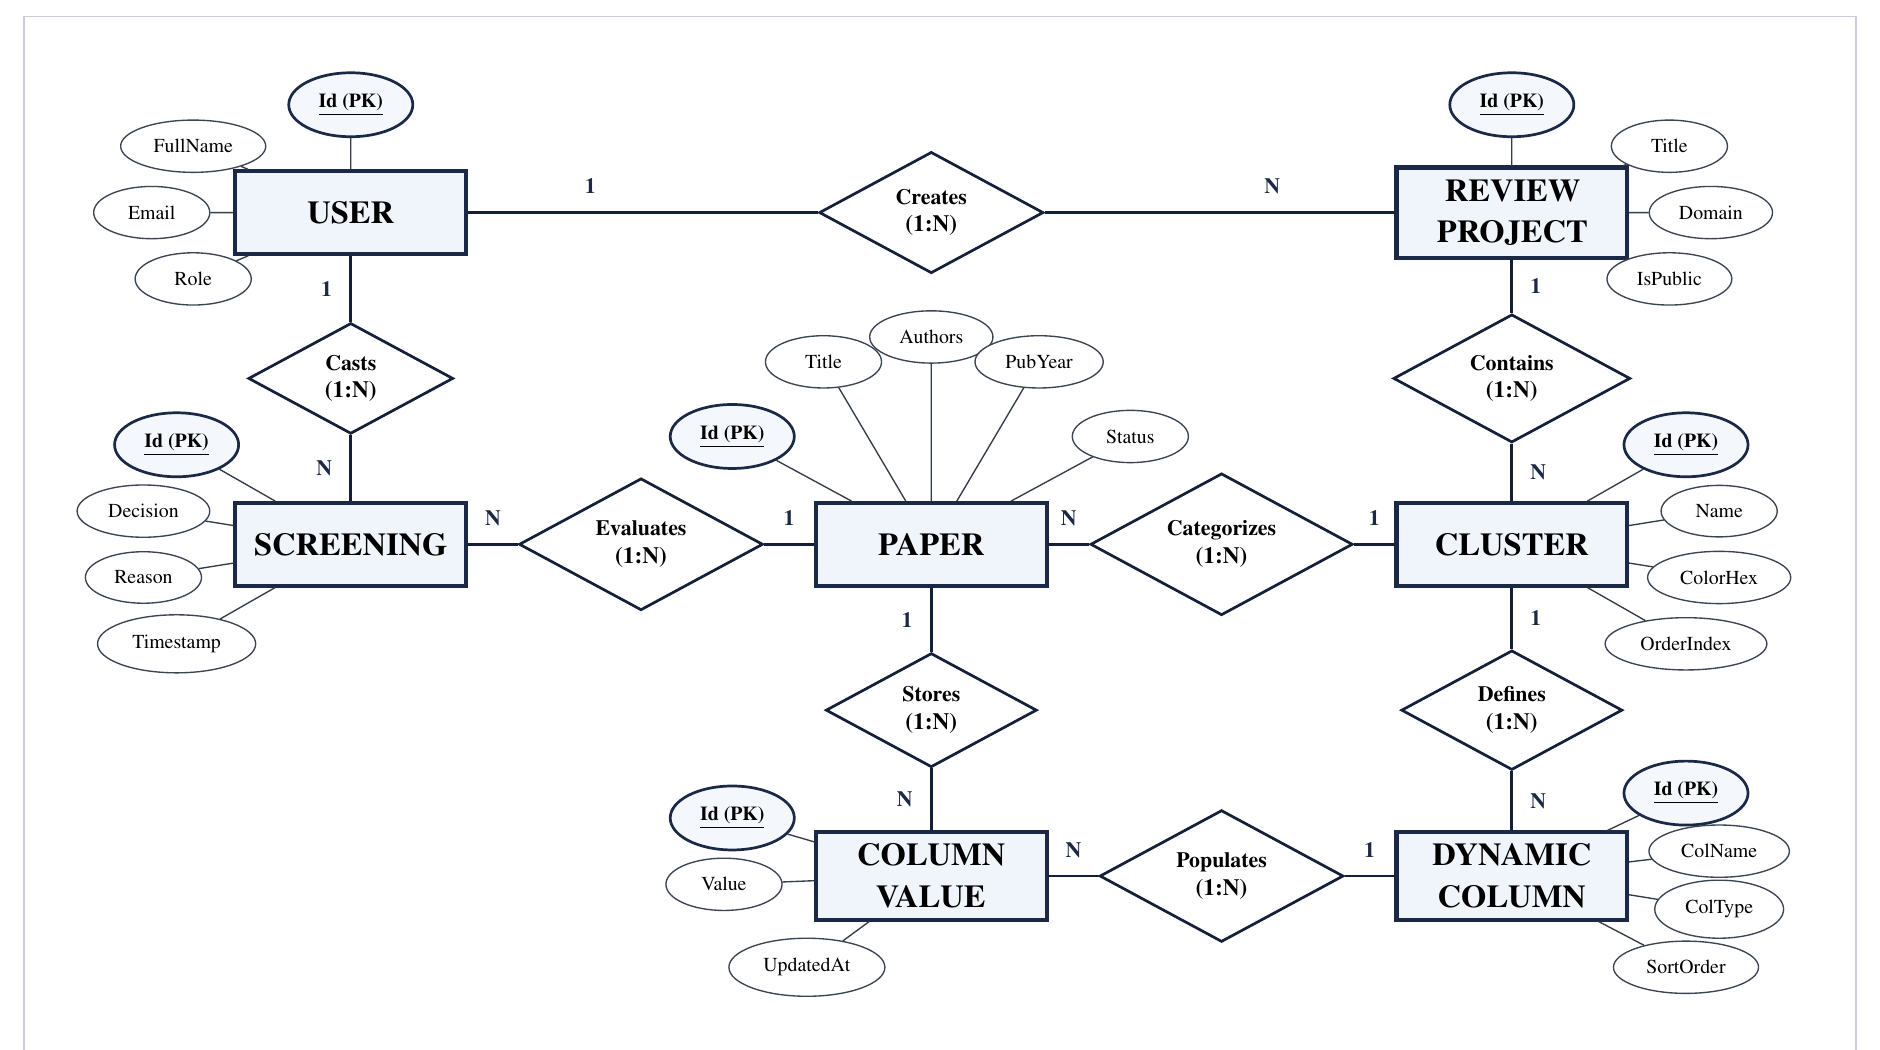
\includegraphics[width=8.0cm, height=5.3cm, keepaspectratio]{figures/diagram_erd.png}%
    }
  \end{column}

  \begin{column}{0.40\textwidth}
    {\fontsize{9pt}{11pt}\selectfont\bfseries\color{DarkText} Relational Architecture}\par\vspace{3pt}
    {\fontsize{7pt}{8.8pt}\selectfont\color{DarkText}
    \begin{itemize}
      \item \textbf{Core Entities:} \texttt{Users}, \texttt{Projects}, \texttt{Papers}, \texttt{Annotations}, \texttt{MatrixRows}, and \texttt{ExtractionFields}.
      \item \textbf{Relational Integrity:} Foreign keys with \texttt{ON DELETE CASCADE} prevent orphan records.
      \item \textbf{Coordinate Storage:} Precise bounding boxes stored as JSON-encoded geometric coordinates.
      \item \textbf{Concurrency Mode:} SQLite WAL enables high-frequency simultaneous reads and writes.
    \end{itemize}}
    
    \vspace{0.35cm}
    \infoCard{5.5cm}{AccentGreen}{Schema Resilience}{ACID Transactions}{%
      Guarantees atomic row updates across concurrent matrix edits.
    }
  \end{column}
\end{columns}
\end{frame}

% ==============================================================================
% SLIDE 17: System Design: Use Case Diagram
% ==============================================================================
\begin{frame}{System Design: Use Case Diagram}
\vspace{-0.25cm}
\begin{columns}[T]
  \begin{column}{0.58\textwidth}
    \centering
    \fboxrule=0.5pt\fboxsep=0pt\fcolorbox{black!15}{white}{%
      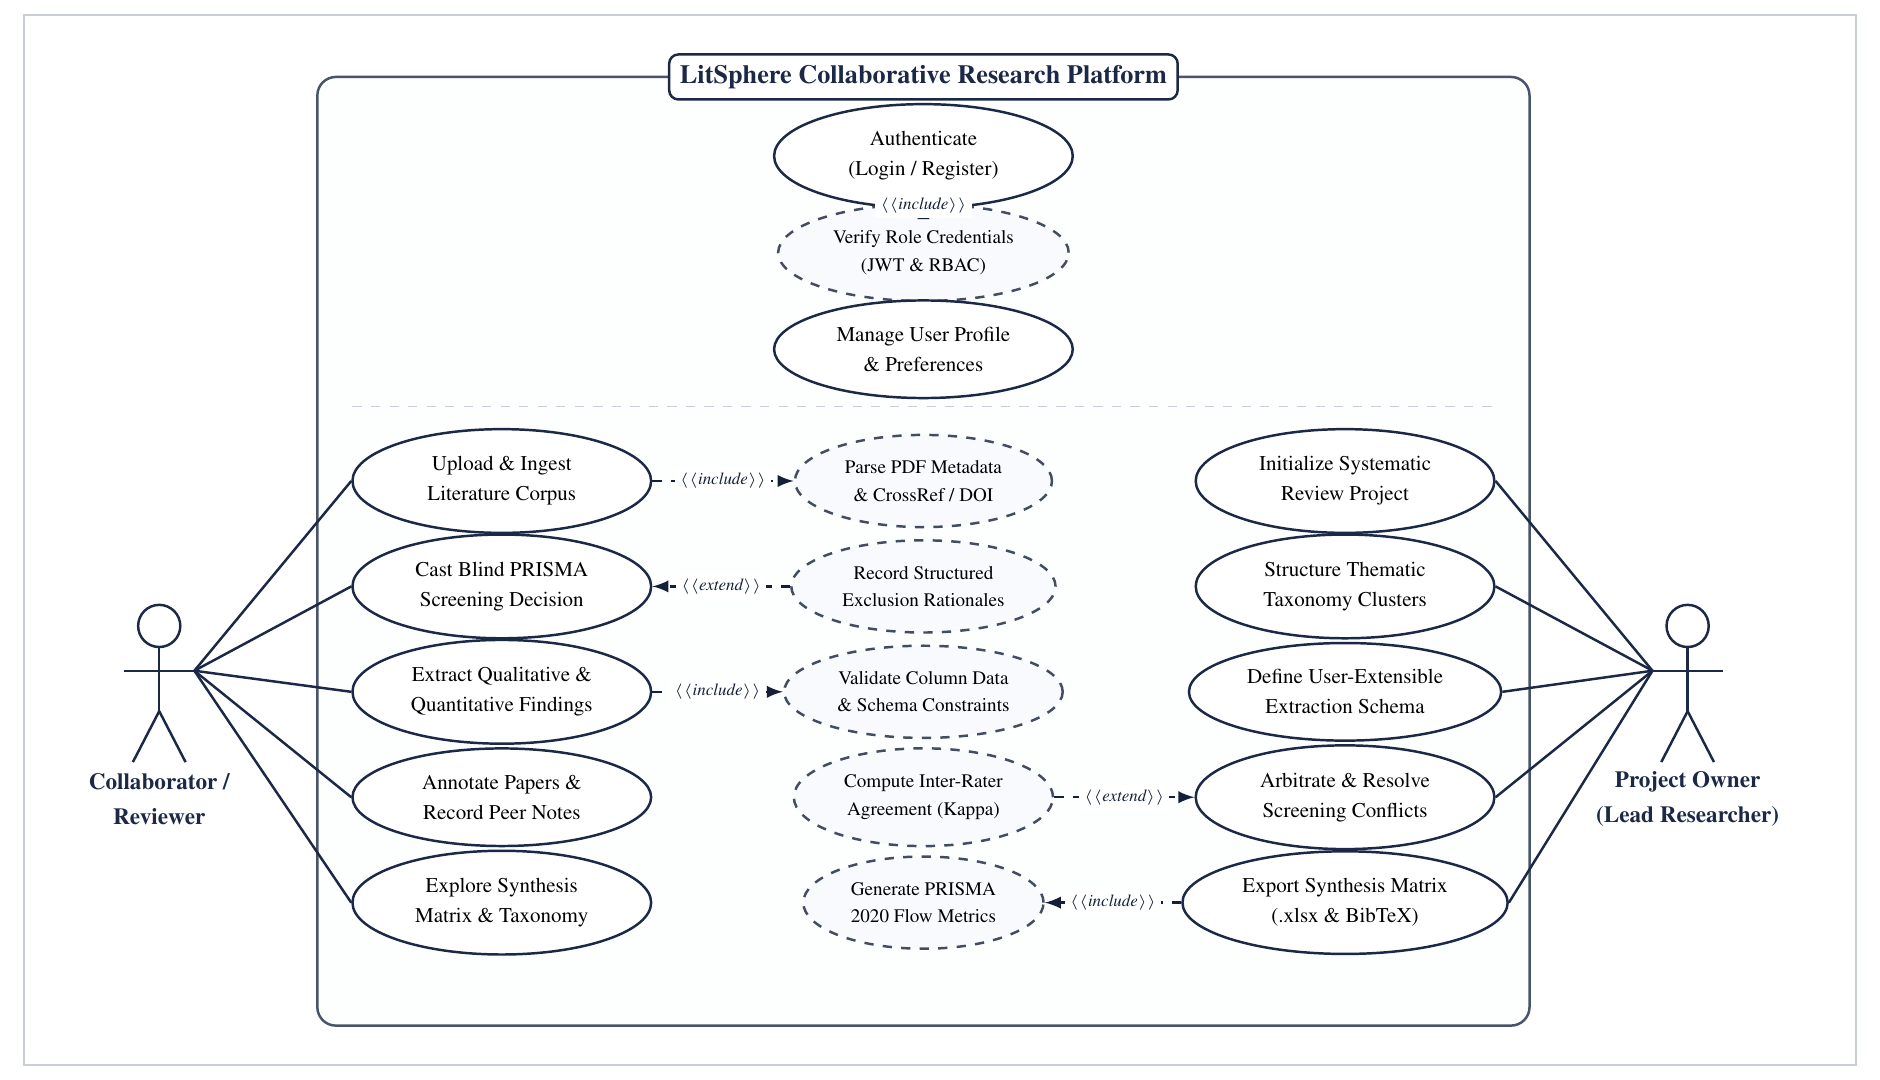
\includegraphics[width=8.0cm, height=5.3cm, keepaspectratio]{figures/diagram_usecase.png}%
    }
  \end{column}

  \begin{column}{0.40\textwidth}
    {\fontsize{9pt}{11pt}\selectfont\bfseries\color{DarkText} Actor \& Role Workflows}\par\vspace{3pt}
    {\fontsize{7pt}{8.8pt}\selectfont\color{DarkText}
    \begin{itemize}
      \item \textbf{Primary Actors:} Researcher (Reviewer), Project Lead (Supervisor), and System Administrator.
      \item \textbf{Researcher Actions:} Ingest papers, highlight text coordinates, extract synthesis variables, and view matrix.
      \item \textbf{Project Lead Actions:} Define research questions, configure extraction schemas, arbitrate conflicts, and export data.
      \item \textbf{Admin Actions:} Manage user accounts, role allocations, system audit logs, and backups.
    \end{itemize}}
    
    \vspace{0.35cm}
    \infoCard{5.5cm}{DarkText}{Role Governance}{RBAC Security}{%
      Enforces strict separation of concerns across review tiers.
    }
  \end{column}
\end{columns}
\end{frame}

% ==============================================================================
% SLIDE 18: UI Screenshots: Live System Demo (Section Breaker - White Theme)
% ==============================================================================
\begin{frame}[plain]
\vspace*{1.3cm}
\begin{center}
  {\fontsize{9.5pt}{12pt}\selectfont\bfseries\color{SubText} SECTION 03}\\[0.35cm]
  {\fontsize{24pt}{28pt}\selectfont\bfseries\color{DarkText} UI Implementation \& Live Demo}\\[0.35cm]
  {\fontsize{11pt}{15pt}\selectfont\color{SubText} Visual Inspection of the Fully Functional LitSphere System}\\[0.45cm]
  {\color{black}\rule{3.5cm}{1.5pt}}
\end{center}
\vfill
\begin{flushright}
  {\fontsize{8pt}{10pt}\selectfont\color{DarkText} \insertframenumber/\inserttotalframenumber\hspace*{0.8cm}}
\end{flushright}
\vspace*{0.15cm}
\end{frame}

% ==============================================================================
% SLIDE 19: UI: User Authentication & Session Login
% ==============================================================================
\begin{frame}{UI: User Authentication \& Session Login}
\vspace{-0.15cm}
\begin{columns}[T]
  \begin{column}{0.48\textwidth}
    \centering
    \fboxrule=0.5pt\fboxsep=0pt\fcolorbox{black!15}{white}{%
      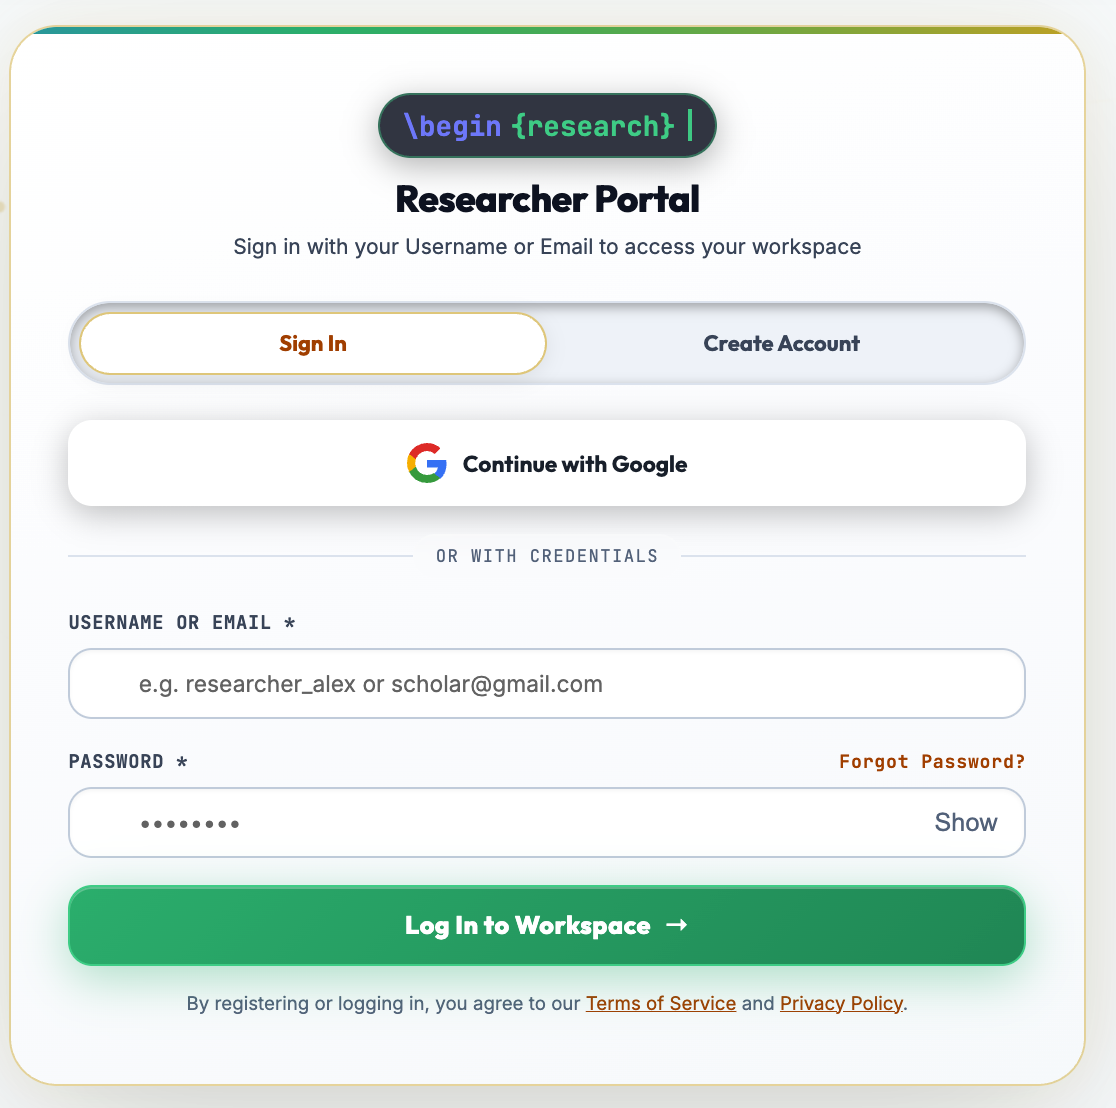
\includegraphics[width=6.8cm, height=5.8cm, keepaspectratio]{figures/ui_01_login.png}%
    }
  \end{column}

  \begin{column}{0.48\textwidth}
    \infoCard{6.8cm}{SubText}{AUTHENTICATION LAYER}{Single-Sign-On \& Session Security}{%
      \begin{itemize}
        \item \textbf{Regex Input Validation:} Instant client-side format checks for academic email addresses and password security.
        \item \textbf{JWT Bearer Generation:} Issues cryptographically signed stateless tokens upon successful credential verification.
        \item \textbf{Bcrypt Hashing:} High-entropy password encryption protecting user accounts from brute-force vectors.
        \item \textbf{Persistent Session State:} Secure local credential caching for seamless navigation across literature workspace tabs.
      \end{itemize}
    }
  \end{column}
\end{columns}
\end{frame}

% ==============================================================================
% SLIDE 20: UI: Researcher Registration & Account Setup
% ==============================================================================
\begin{frame}{UI: Researcher Registration \& Account Setup}
\vspace{-0.15cm}
\begin{columns}[T]
  \begin{column}{0.48\textwidth}
    \centering
    \fboxrule=0.5pt\fboxsep=0pt\fcolorbox{black!15}{white}{%
      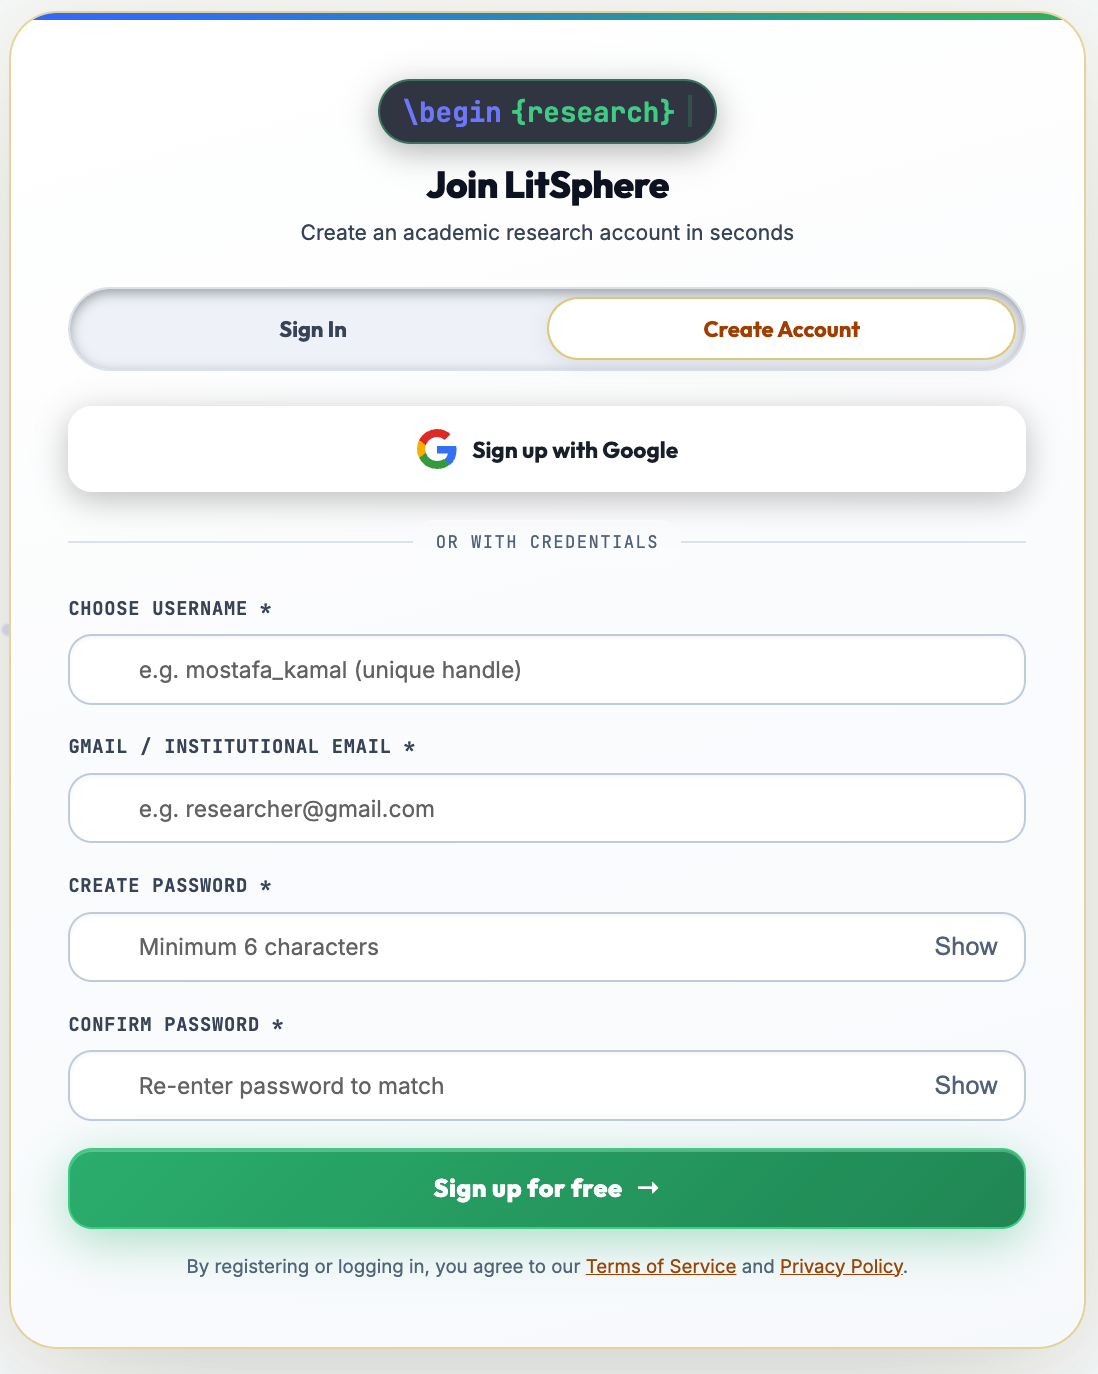
\includegraphics[width=6.8cm, height=5.8cm, keepaspectratio]{figures/ui_02_create_account.png}%
    }
  \end{column}

  \begin{column}{0.48\textwidth}
    \infoCard{6.8cm}{SubText}{USER ONBOARDING}{Institutional Registration \& Role Assignment}{%
      \begin{itemize}
        \item \textbf{Academic Profile Capture:} Records researcher full name, department, and university affiliation during signup.
        \item \textbf{Role-Based Governance:} Grants initial access tiers (Student Researcher, Reviewer, or Principal Investigator).
        \item \textbf{Password Policy Enforcement:} Multi-condition character validation ensures robust credential security.
        \item \textbf{Immediate Workspace Access:} Direct transition into systematic literature review projects without manual activation lag.
      \end{itemize}
    }
  \end{column}
\end{columns}
\end{frame}

% ==============================================================================
% SLIDE 21: UI: Researcher Profile & Institutional Affiliation
% ==============================================================================
\begin{frame}{UI: Researcher Profile \& Institutional Affiliation}
\vspace{-0.20cm}
\centering
\fboxrule=0.5pt\fboxsep=0pt\fcolorbox{black!15}{white}{%
  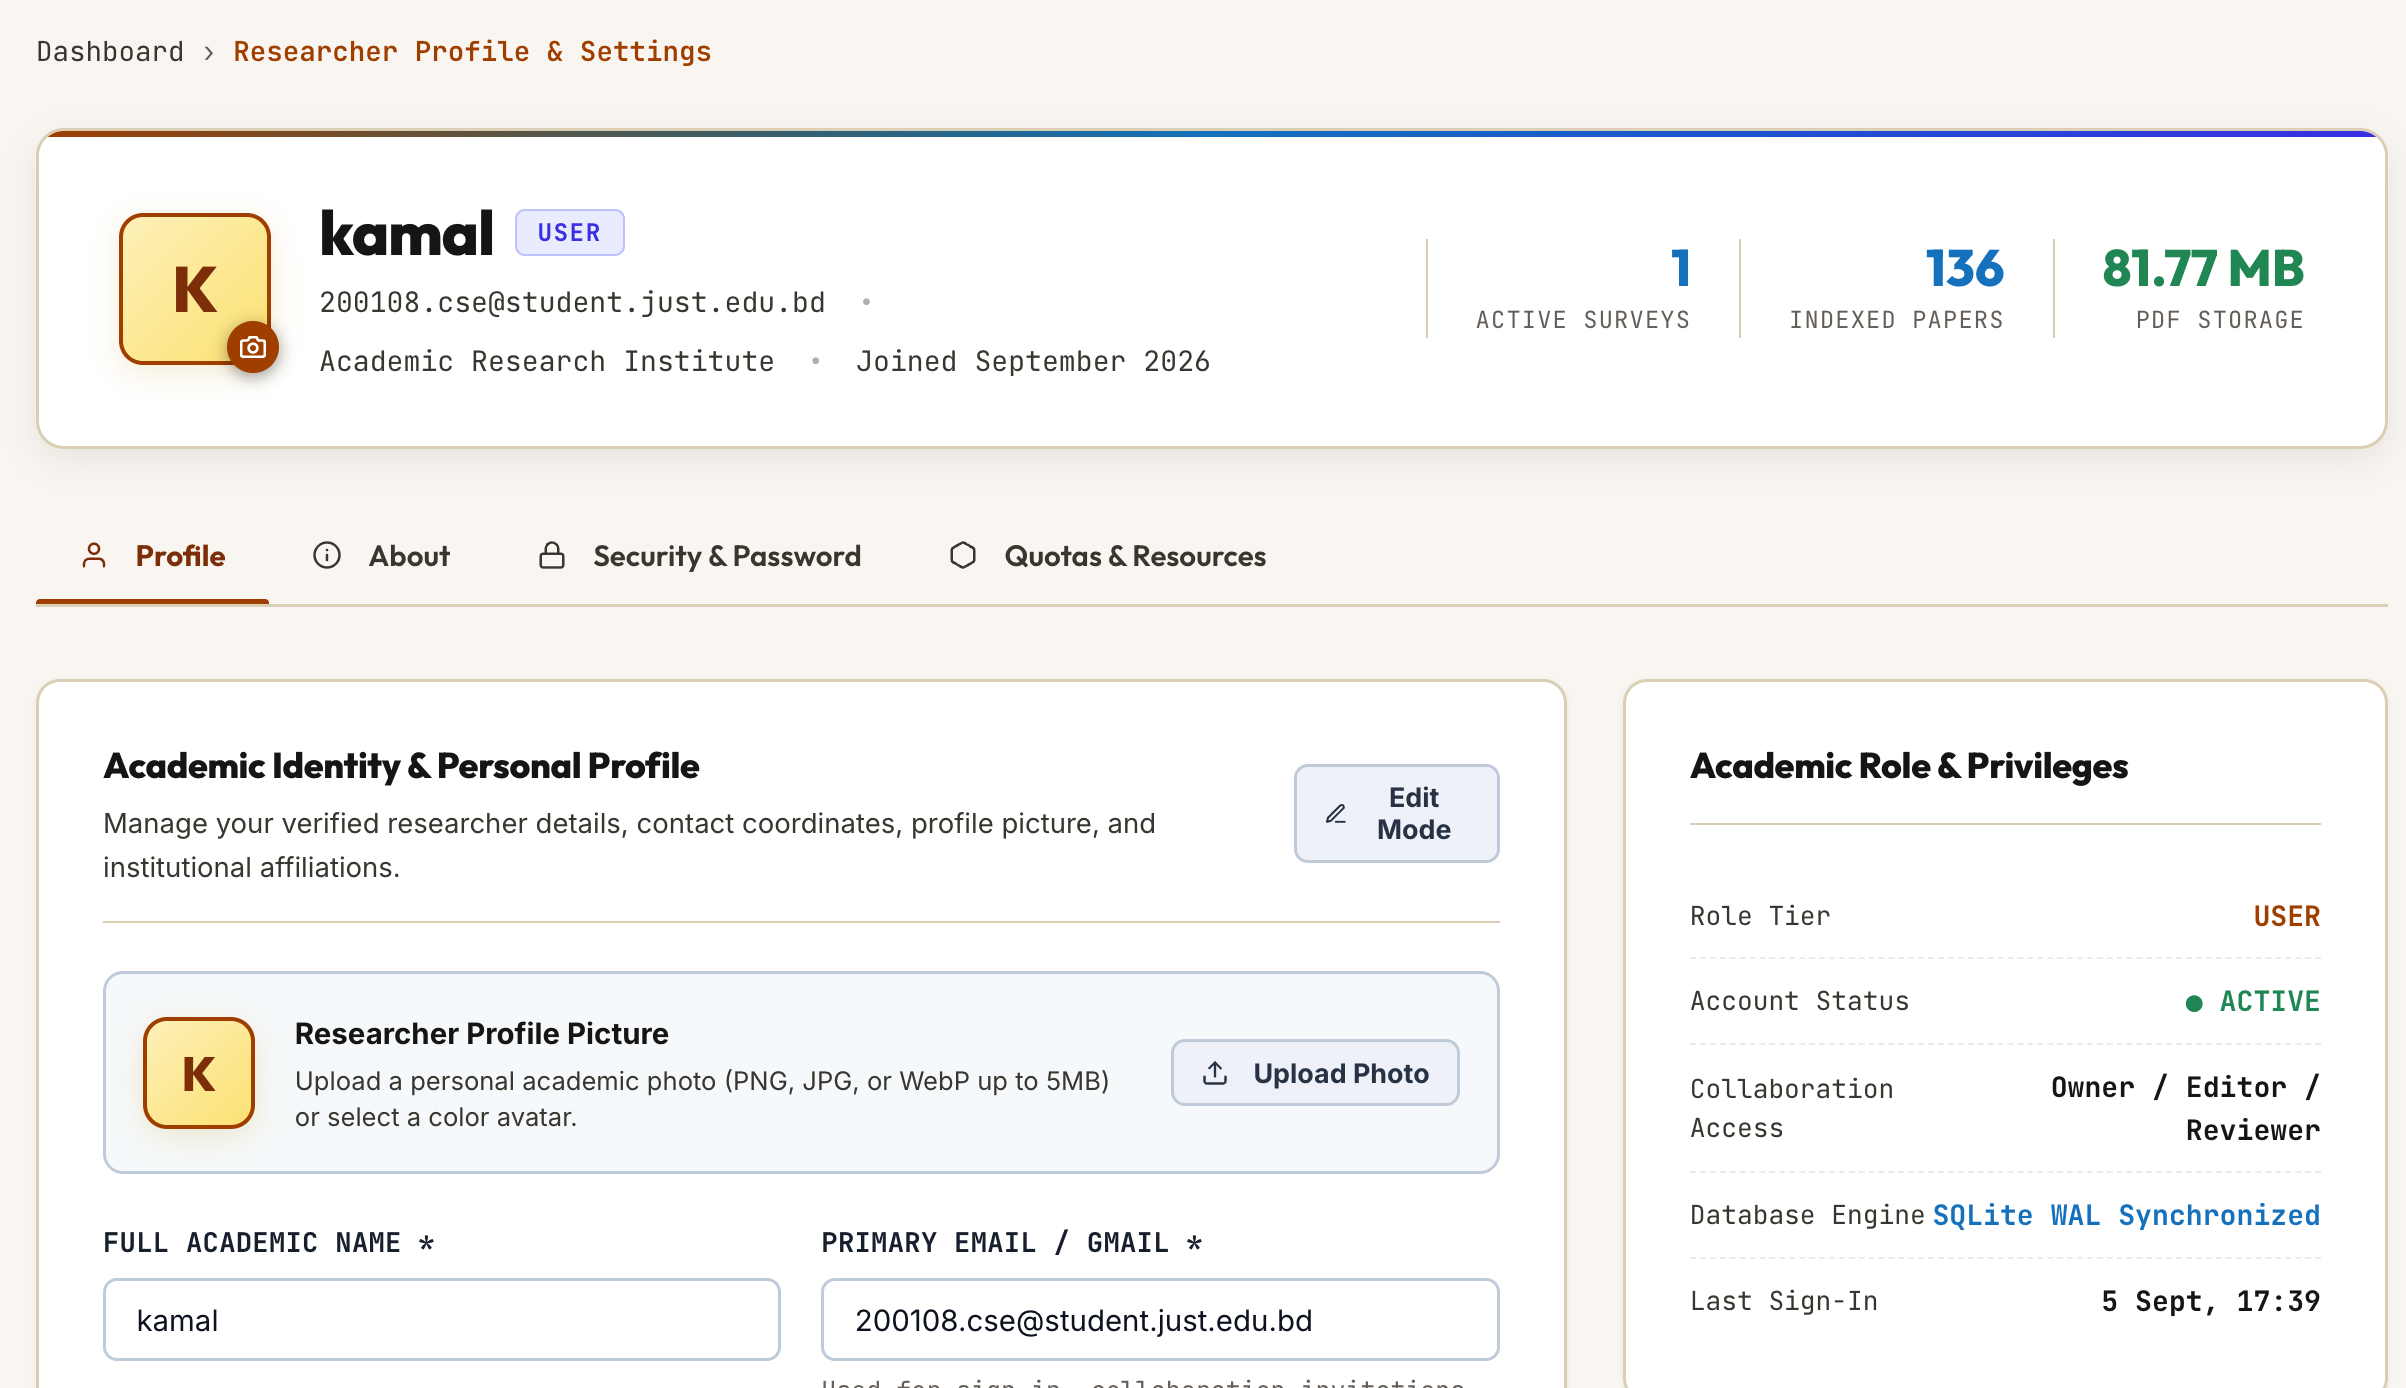
\includegraphics[width=13.6cm, height=3.80cm, keepaspectratio]{figures/ui_03_user_profile.png}%
}
\par\vspace{0.18cm}
\begin{columns}[T]
  \begin{column}{0.48\textwidth}
    \infoCard{6.8cm}{SubText}{ROLE GOVERNANCE}{Account Credentials \& Access Roles}{%
      Displays active identity credentials, institutional department metadata, and user privileges across all assigned review teams.
    }
  \end{column}

  \begin{column}{0.48\textwidth}
    \infoCard{6.8cm}{SubText}{ACTIVITY TELEMETRY}{Project Memberships \& Contributions}{%
      Monitors active literature survey projects, tracks individual paper extraction tallies, and manages password updates.
    }
  \end{column}
\end{columns}
\end{frame}

% ==============================================================================
% SLIDE 22: UI: Central Project Dashboard & Review Metrics
% ==============================================================================
\begin{frame}{UI: Project Dashboard \& Review Metrics}
\vspace{-0.20cm}
\centering
\fboxrule=0.5pt\fboxsep=0pt\fcolorbox{black!15}{white}{%
  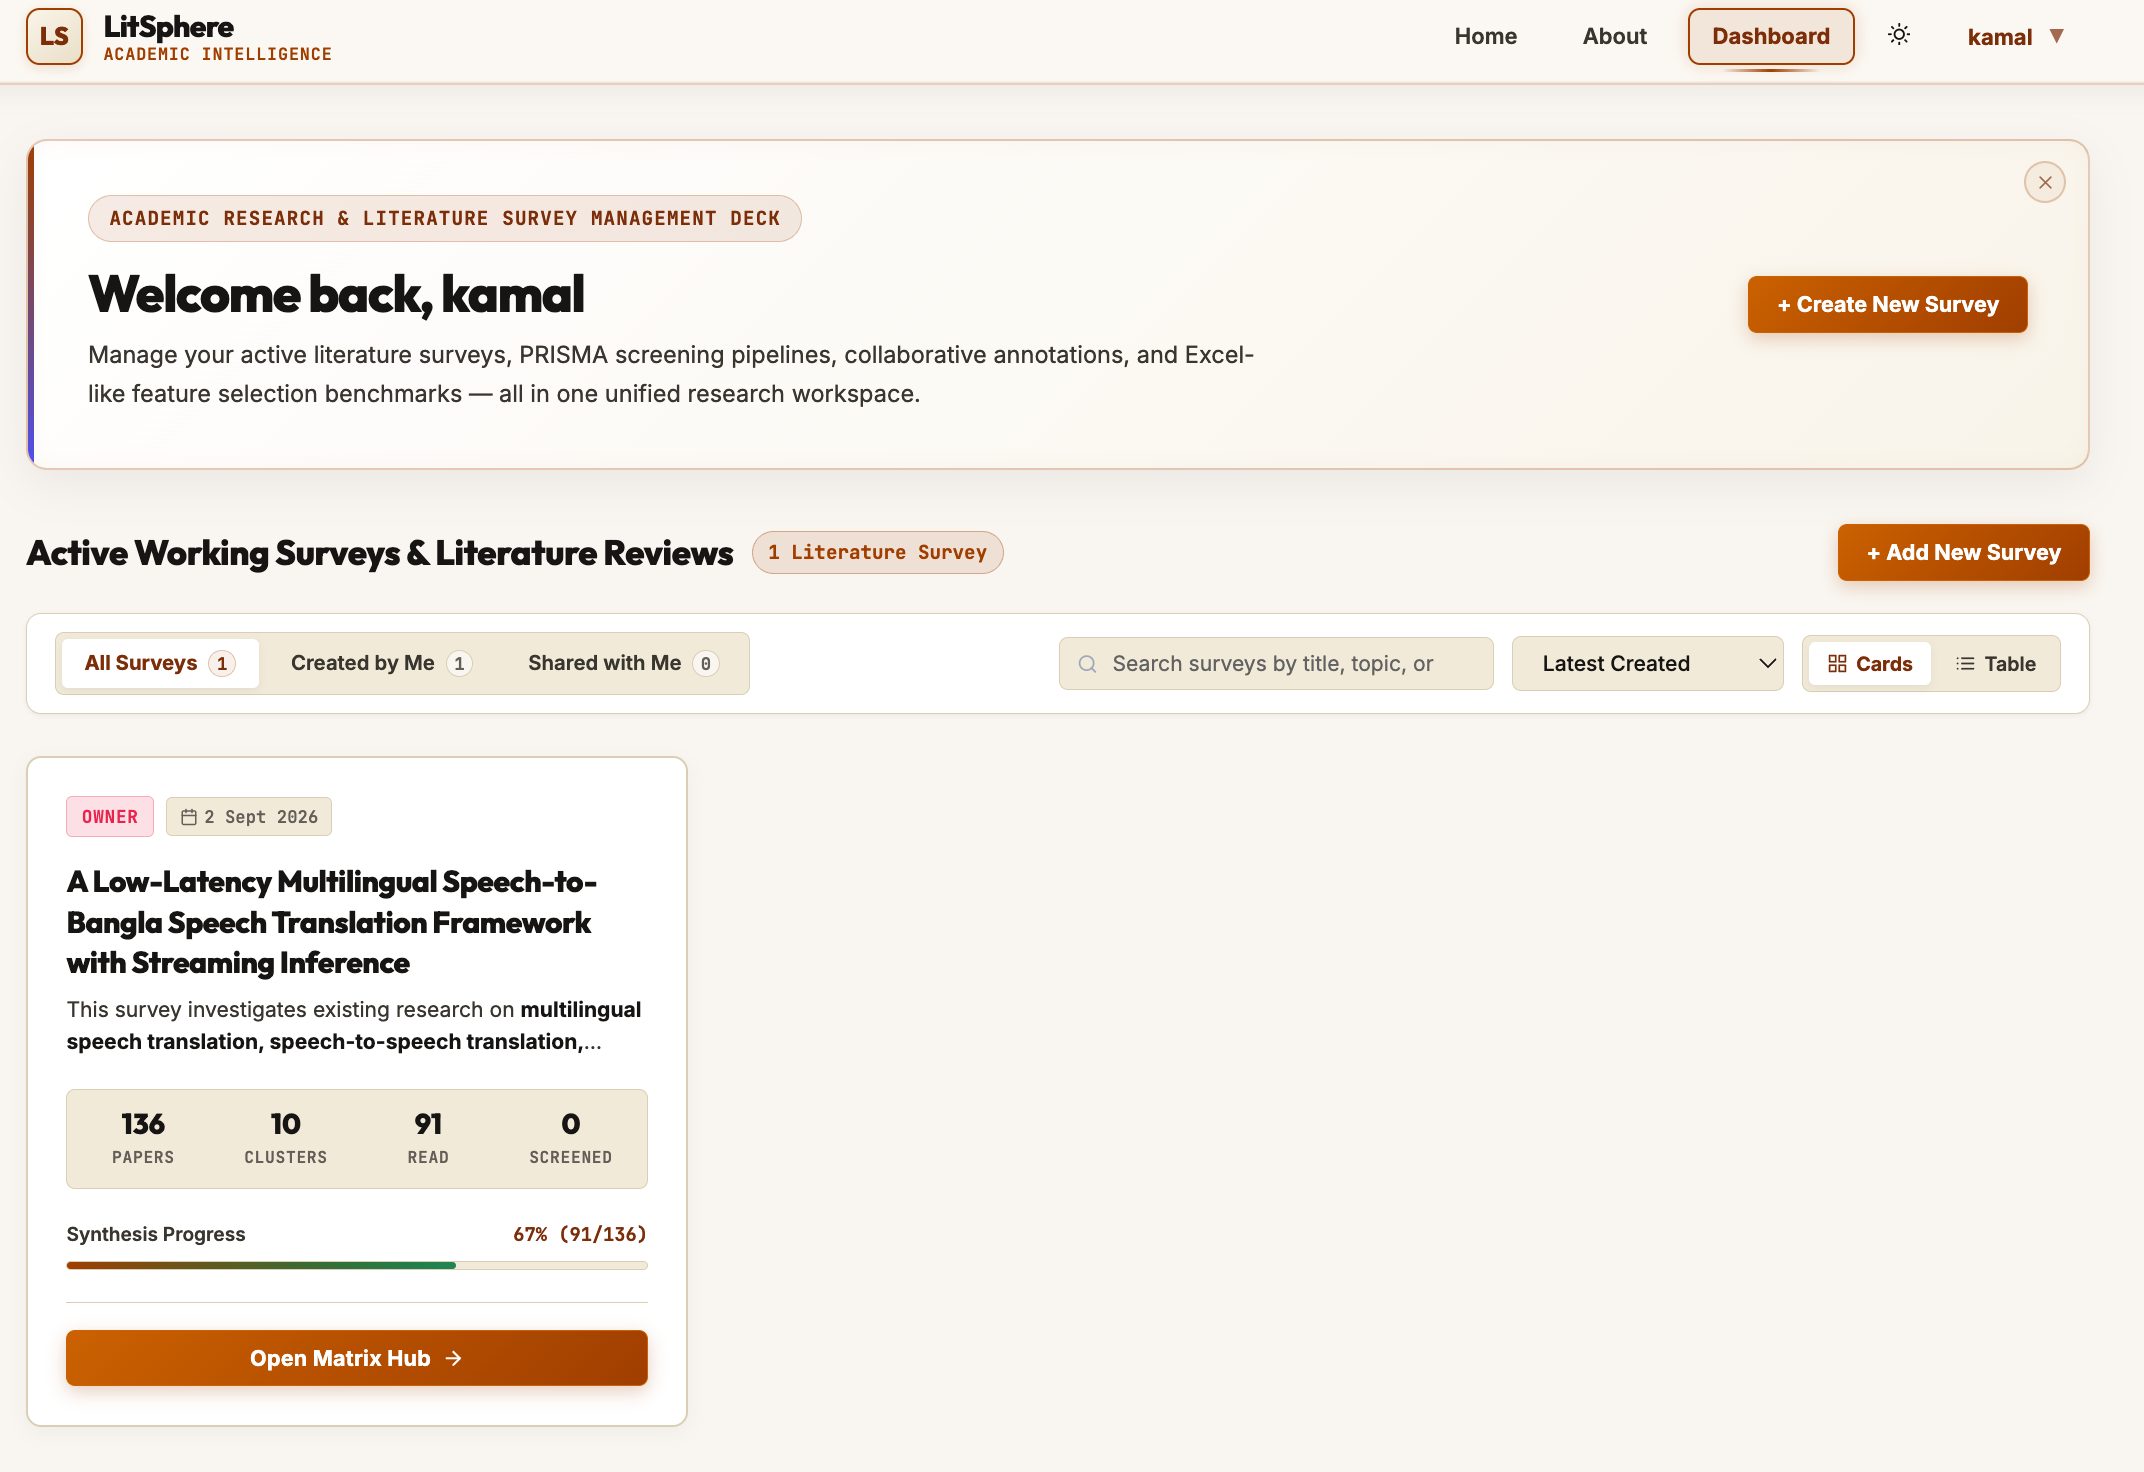
\includegraphics[width=13.6cm, height=3.80cm, keepaspectratio]{figures/ui_04_dashboard.png}%
}
\par\vspace{0.18cm}
\begin{columns}[T]
  \begin{column}{0.48\textwidth}
    \infoCard{6.8cm}{SubText}{EXECUTIVE METRICS}{Survey Portfolio \& Extraction KPIs}{%
      Real-time operational dashboard providing high-level progress tracking, paper ingestion counts, and variable extraction status.
    }
  \end{column}

  \begin{column}{0.48\textwidth}
    \infoCard{6.8cm}{SubText}{WORKFLOW ACTIONS}{Protocol Launch \& Batch Ingestion}{%
      One-click shortcuts to initiate new PRISMA literature review protocols, import BibTeX bibliographic libraries, and add collaborators.
    }
  \end{column}
\end{columns}
\end{frame}

% ==============================================================================
% SLIDE 23: UI: Survey Project Workspace & Paper Ingestion
% ==============================================================================
\begin{frame}{UI: Survey Workspace \& Literature Ingestion}
\vspace{-0.20cm}
\centering
\fboxrule=0.5pt\fboxsep=0pt\fcolorbox{black!15}{white}{%
  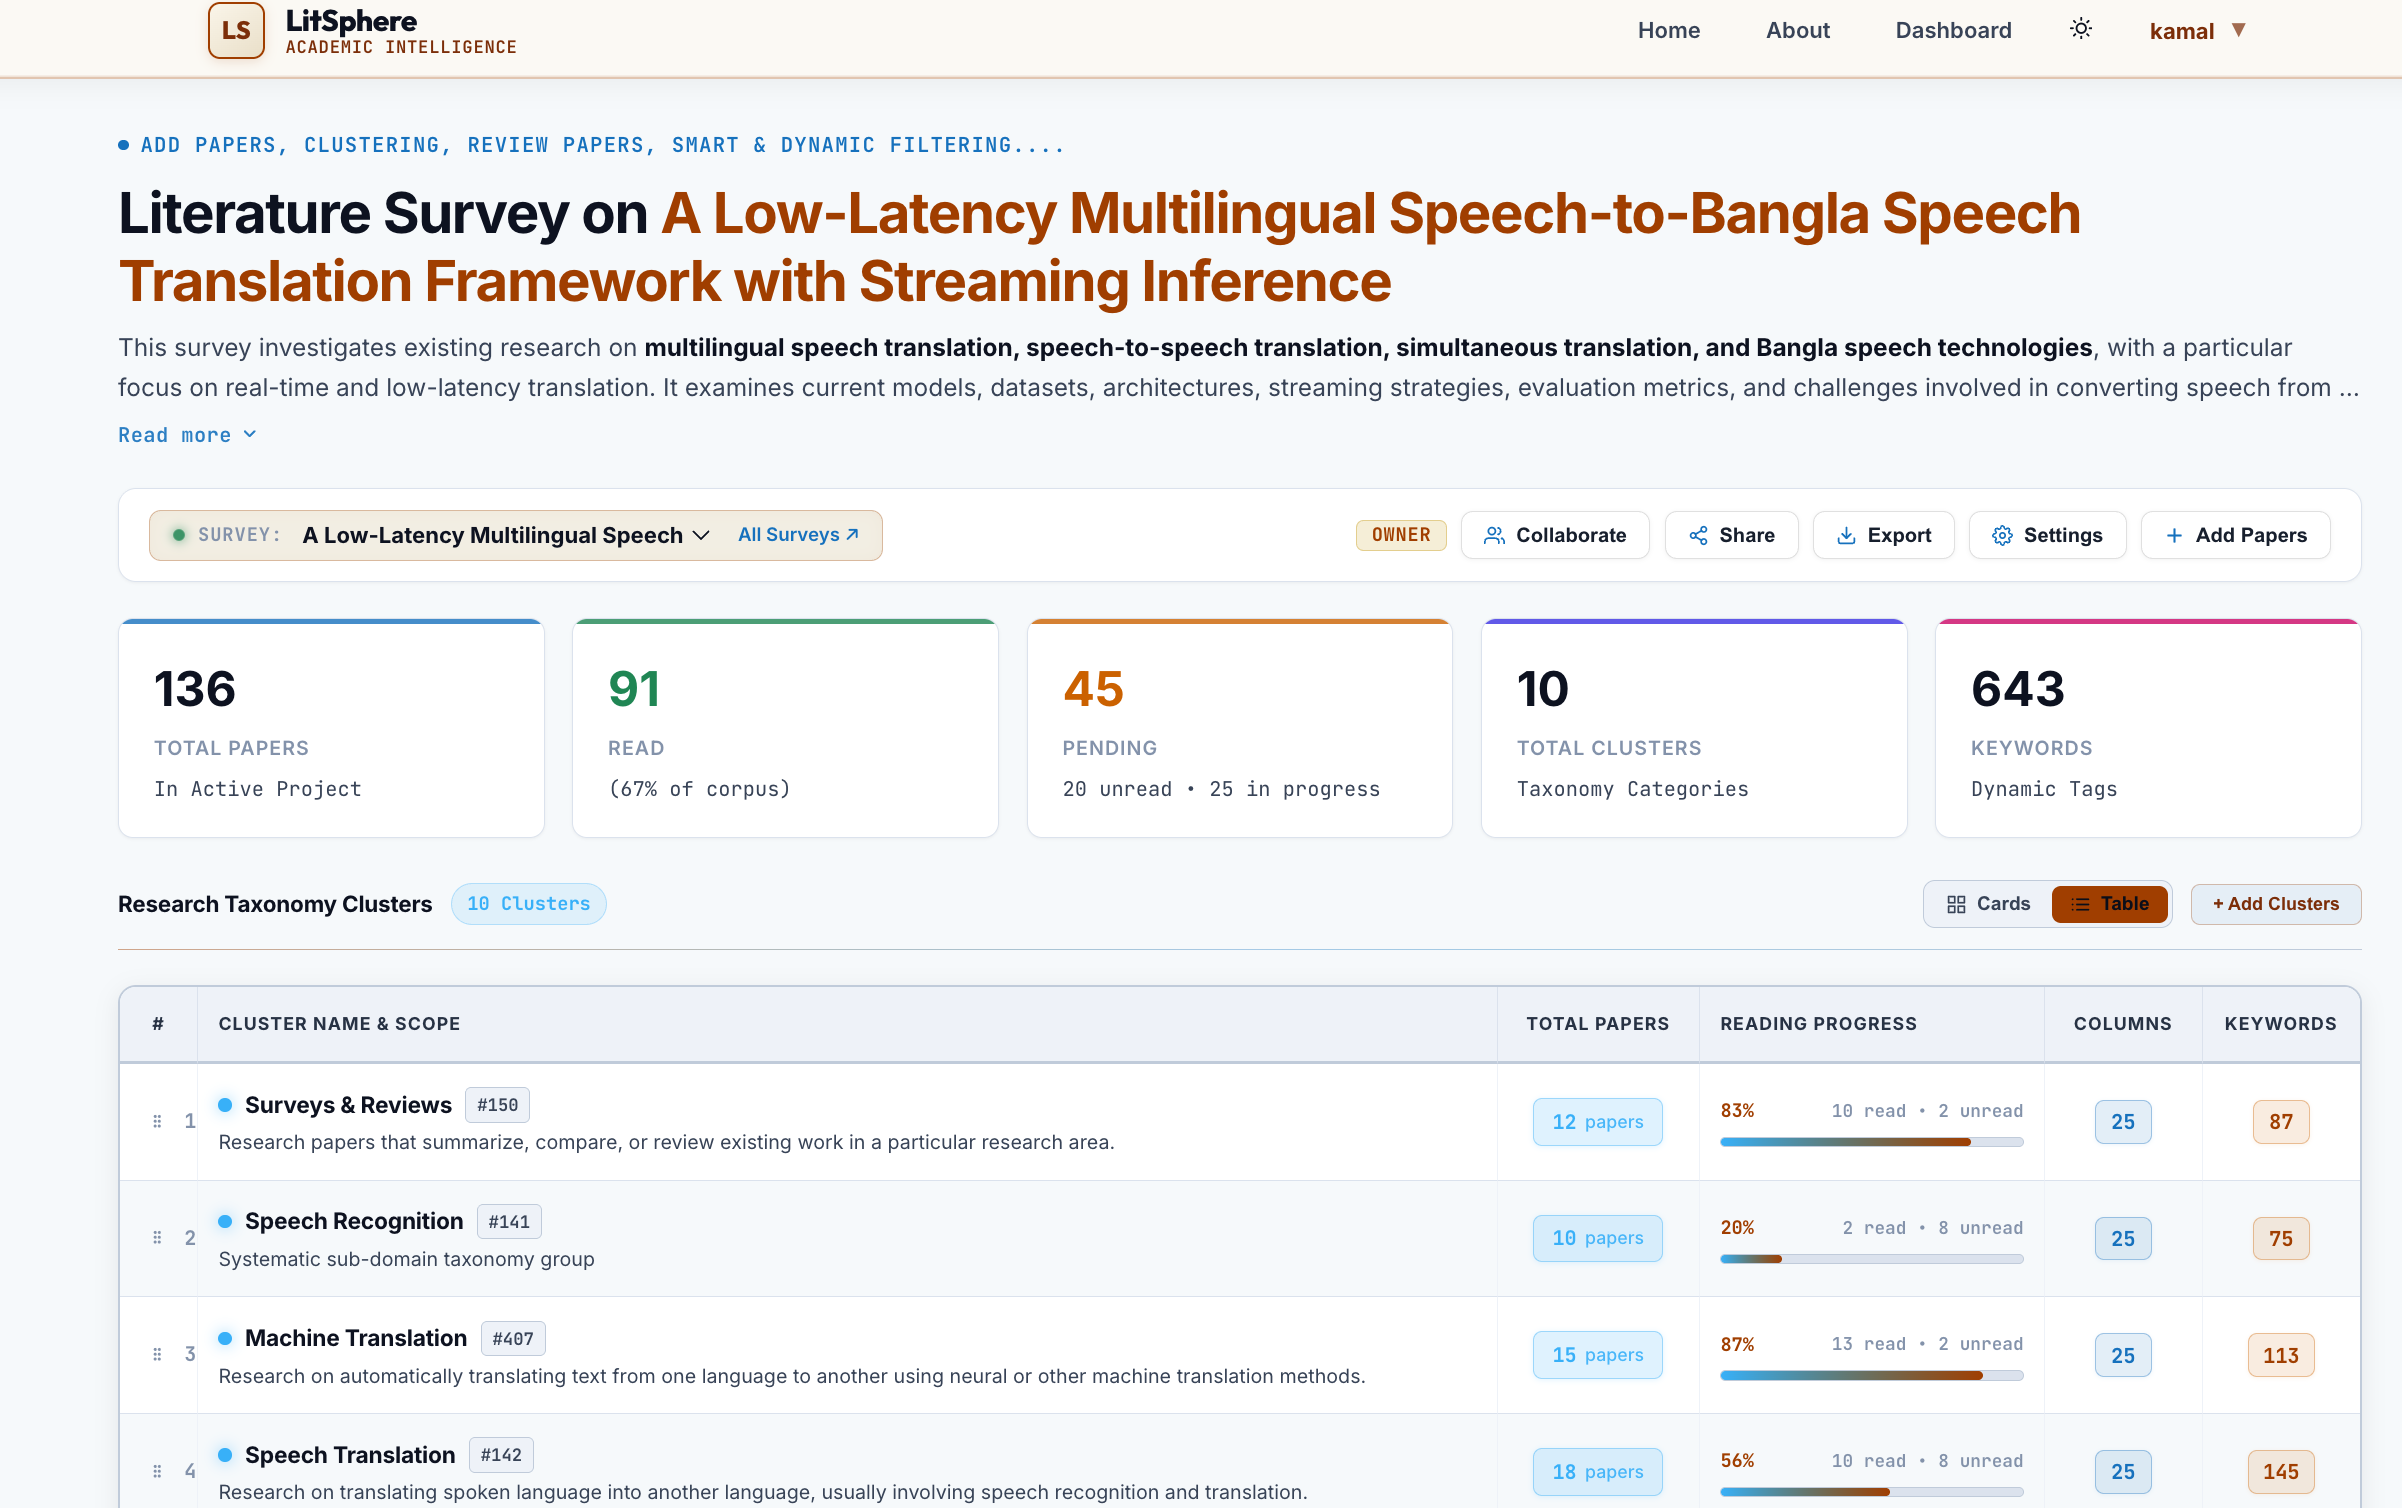
\includegraphics[width=13.6cm, height=3.80cm, keepaspectratio]{figures/ui_05_workspace.png}%
}
\par\vspace{0.18cm}
\begin{columns}[T]
  \begin{column}{0.48\textwidth}
    \infoCard{6.8cm}{SubText}{INGESTION PIPELINE}{Drag-and-Drop Batch File Upload}{%
      High-throughput multi-file PDF ingestion interface with automated bibliographic parsing, title hashing, and metadata normalization.
    }
  \end{column}

  \begin{column}{0.48\textwidth}
    \infoCard{6.8cm}{SubText}{LITERATURE CATALOG}{Status Filtering \& Review Queue}{%
      Organized research repository featuring status pills (Uploaded, In Progress, Synthesized) and multi-field keyword filtering.
    }
  \end{column}
\end{columns}
\end{frame}

% ==============================================================================
% SLIDE 24: UI: Split-Screen Dual-Pane Paper Reviewer
% ==============================================================================
\begin{frame}{UI: Split-Screen Dual-Pane Paper Reviewer}
\vspace{-0.20cm}
\centering
\fboxrule=0.5pt\fboxsep=0pt\fcolorbox{black!15}{white}{%
  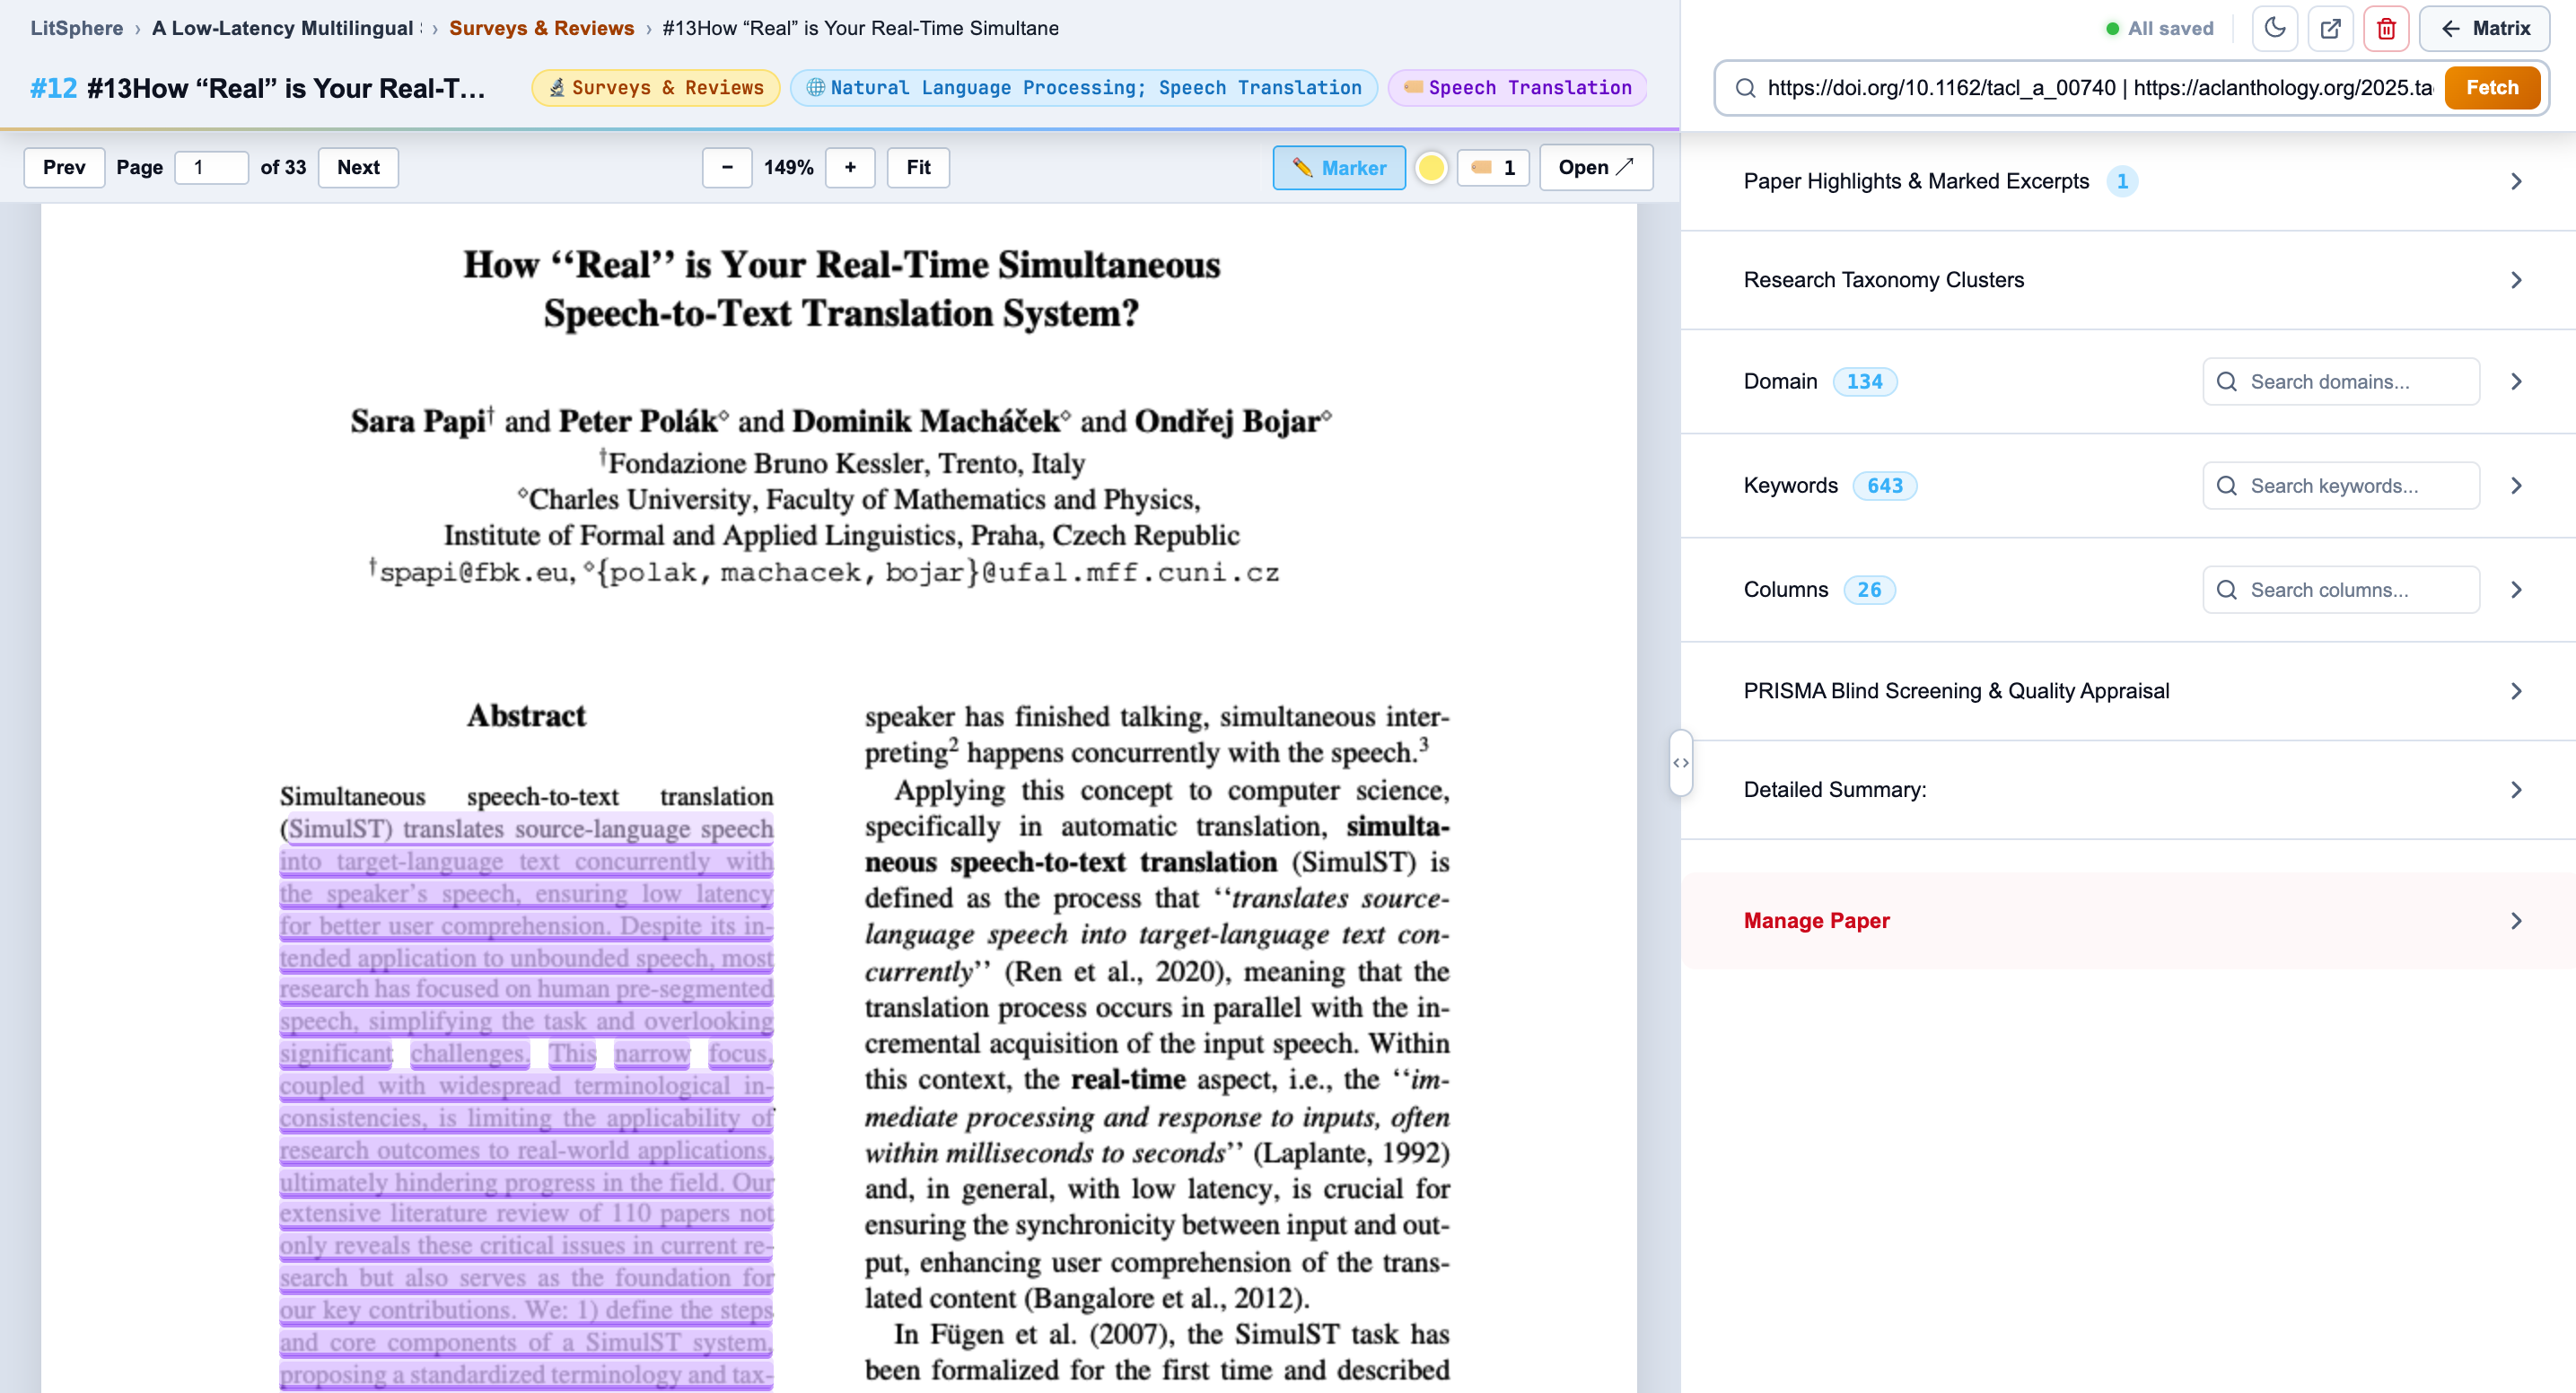
\includegraphics[width=13.6cm, height=3.80cm, keepaspectratio]{figures/ui_06_reviewer.png}%
}
\par\vspace{0.18cm}
\begin{columns}[T]
  \begin{column}{0.48\textwidth}
    \infoCard{6.8cm}{SubText}{DUAL-PANE WORKSPACE}{Synchronous In-Browser PDF Reading}{%
      Integrated PDF reader docked side-by-side with extraction inputs, eliminating workflow disruption from external desktop viewers.
    }
  \end{column}

  \begin{column}{0.48\textwidth}
    \infoCard{6.8cm}{SubText}{COORDINATE ANCHORING}{Geometric BBox Text Highlighting}{%
      Text selections capture exact normalized bounding-box coordinates, providing direct jump-to-quote verification in under 2 seconds.
    }
  \end{column}
\end{columns}
\end{frame}

% ==============================================================================
% SLIDE 25: UI: Interactive Master Synthesis Matrix Grid
% ==============================================================================
\begin{frame}{UI: Interactive Master Synthesis Matrix Grid}
\vspace{-0.20cm}
\centering
\fboxrule=0.5pt\fboxsep=0pt\fcolorbox{black!15}{white}{%
  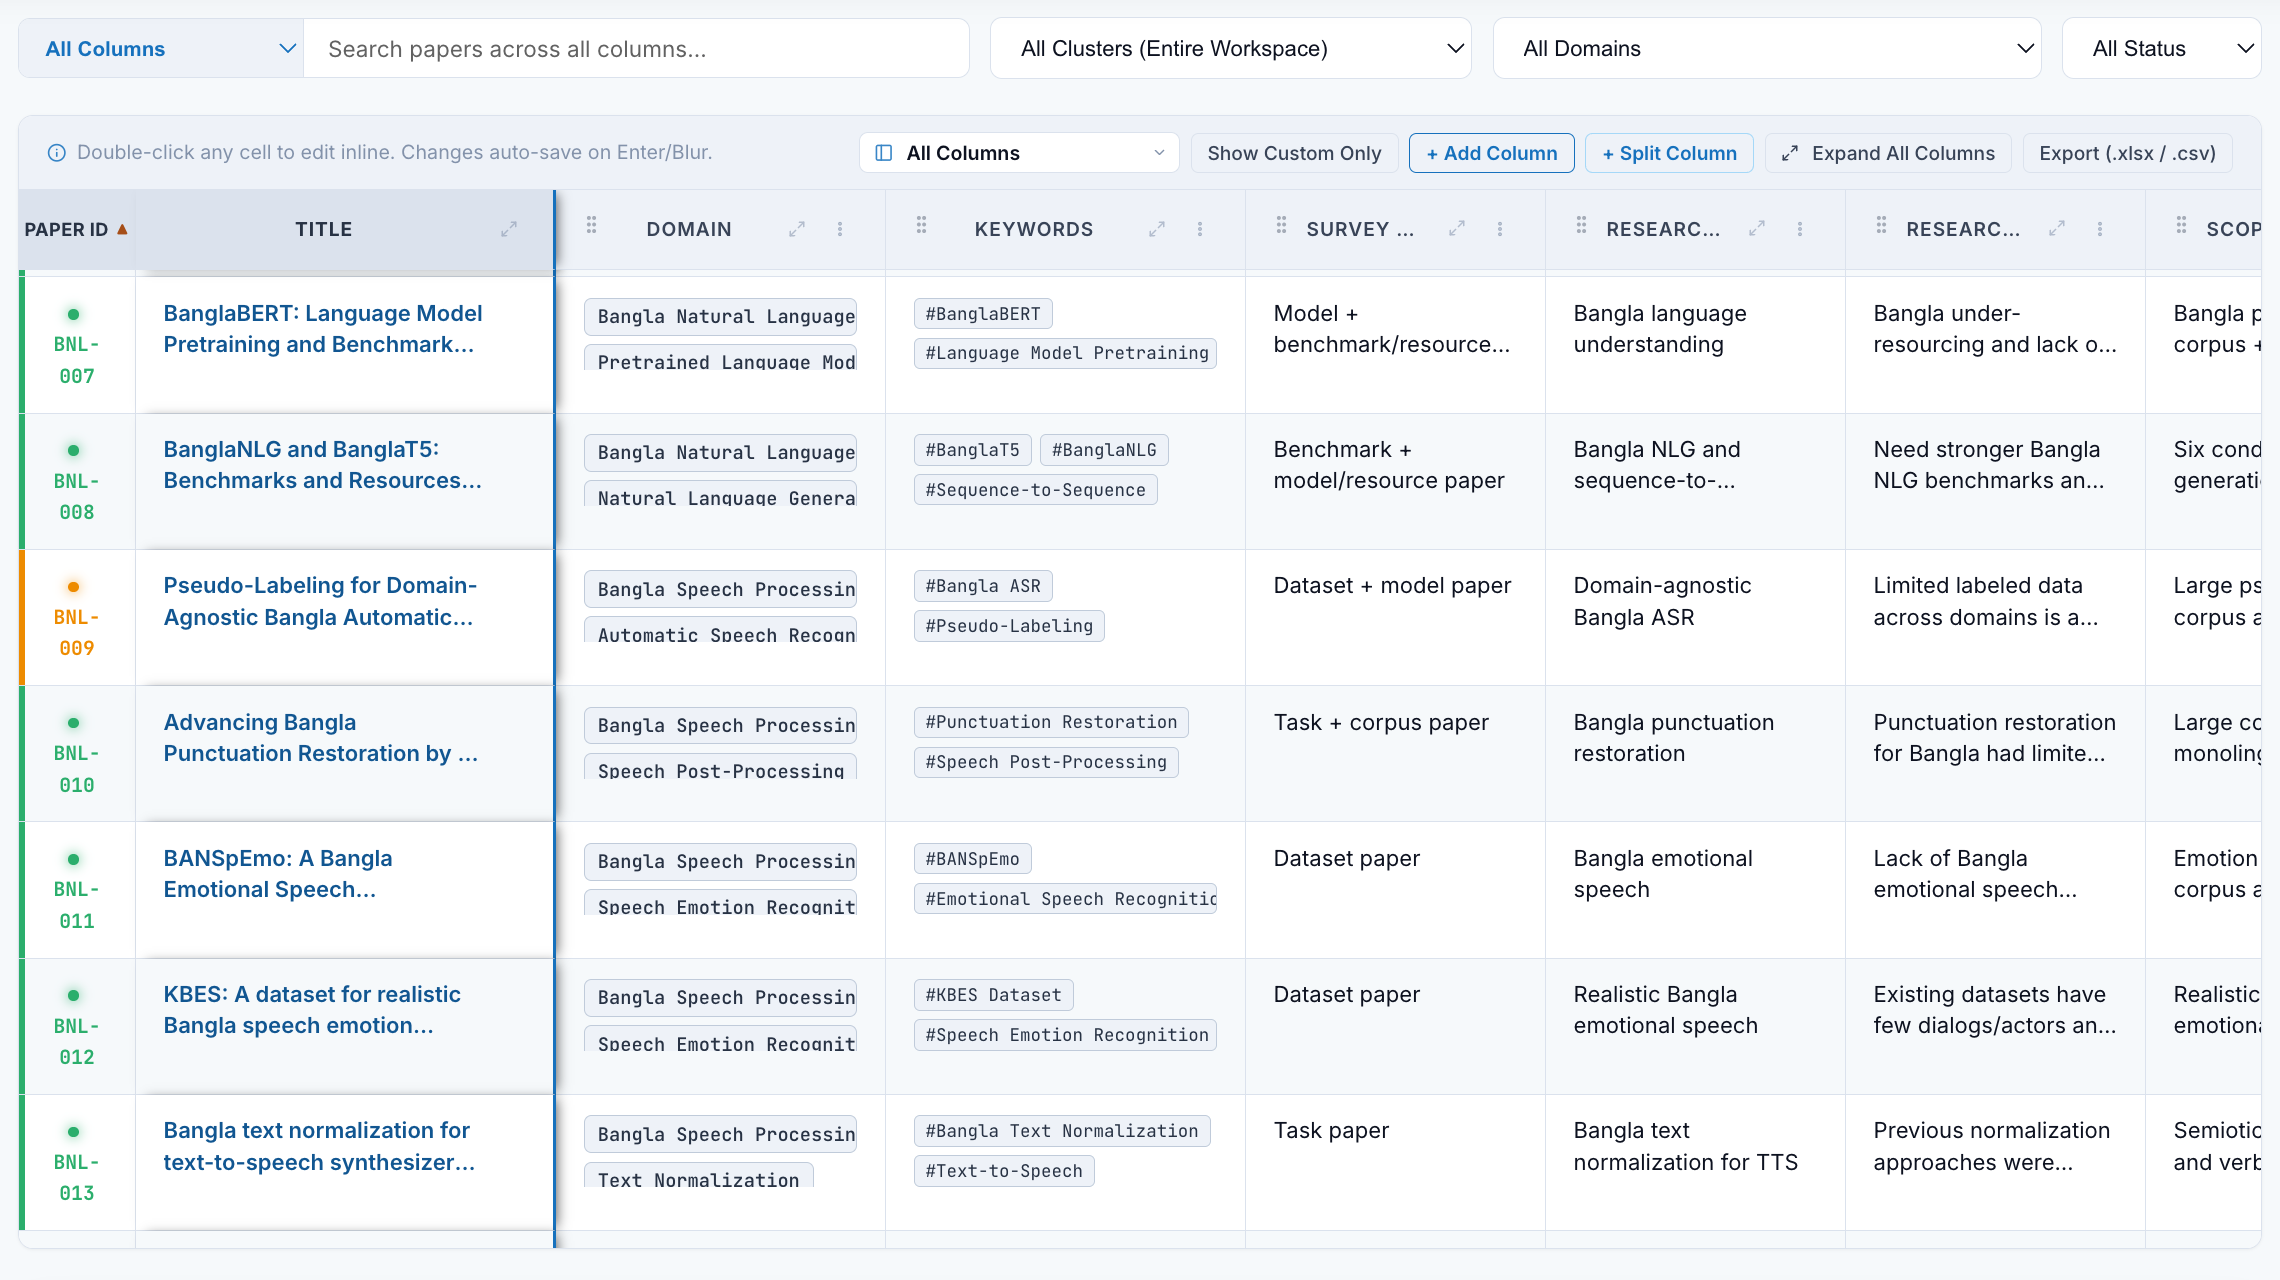
\includegraphics[width=13.6cm, height=3.80cm, keepaspectratio]{figures/ui_07_matrix.png}%
}
\par\vspace{0.18cm}
\begin{columns}[T]
  \begin{column}{0.48\textwidth}
    \infoCard{6.8cm}{SubText}{CROSS-STUDY SYNTHESIS}{Consolidated Comparative Grid}{%
      Multi-dimensional tabular matrix harmonizing extracted variables (methodology, datasets, metrics, limitations) across all papers.
    }
  \end{column}

  \begin{column}{0.48\textwidth}
    \infoCard{6.8cm}{SubText}{TRANSACTIONAL EXPORT}{Inline Editing \& 1-Click LaTeX}{%
      Supports real-time inline updates with ACID database guarantees, plus direct 1-click export to publication-ready LaTeX booktabs code.
    }
  \end{column}
\end{columns}
\end{frame}

% ==============================================================================
% SLIDE 26: UI: Thematic Clustering & Synthesis Taxonomy
% ==============================================================================
\begin{frame}{UI: Thematic Clustering \& Synthesis Taxonomy}
\vspace{-0.20cm}
\centering
\fboxrule=0.5pt\fboxsep=0pt\fcolorbox{black!15}{white}{%
  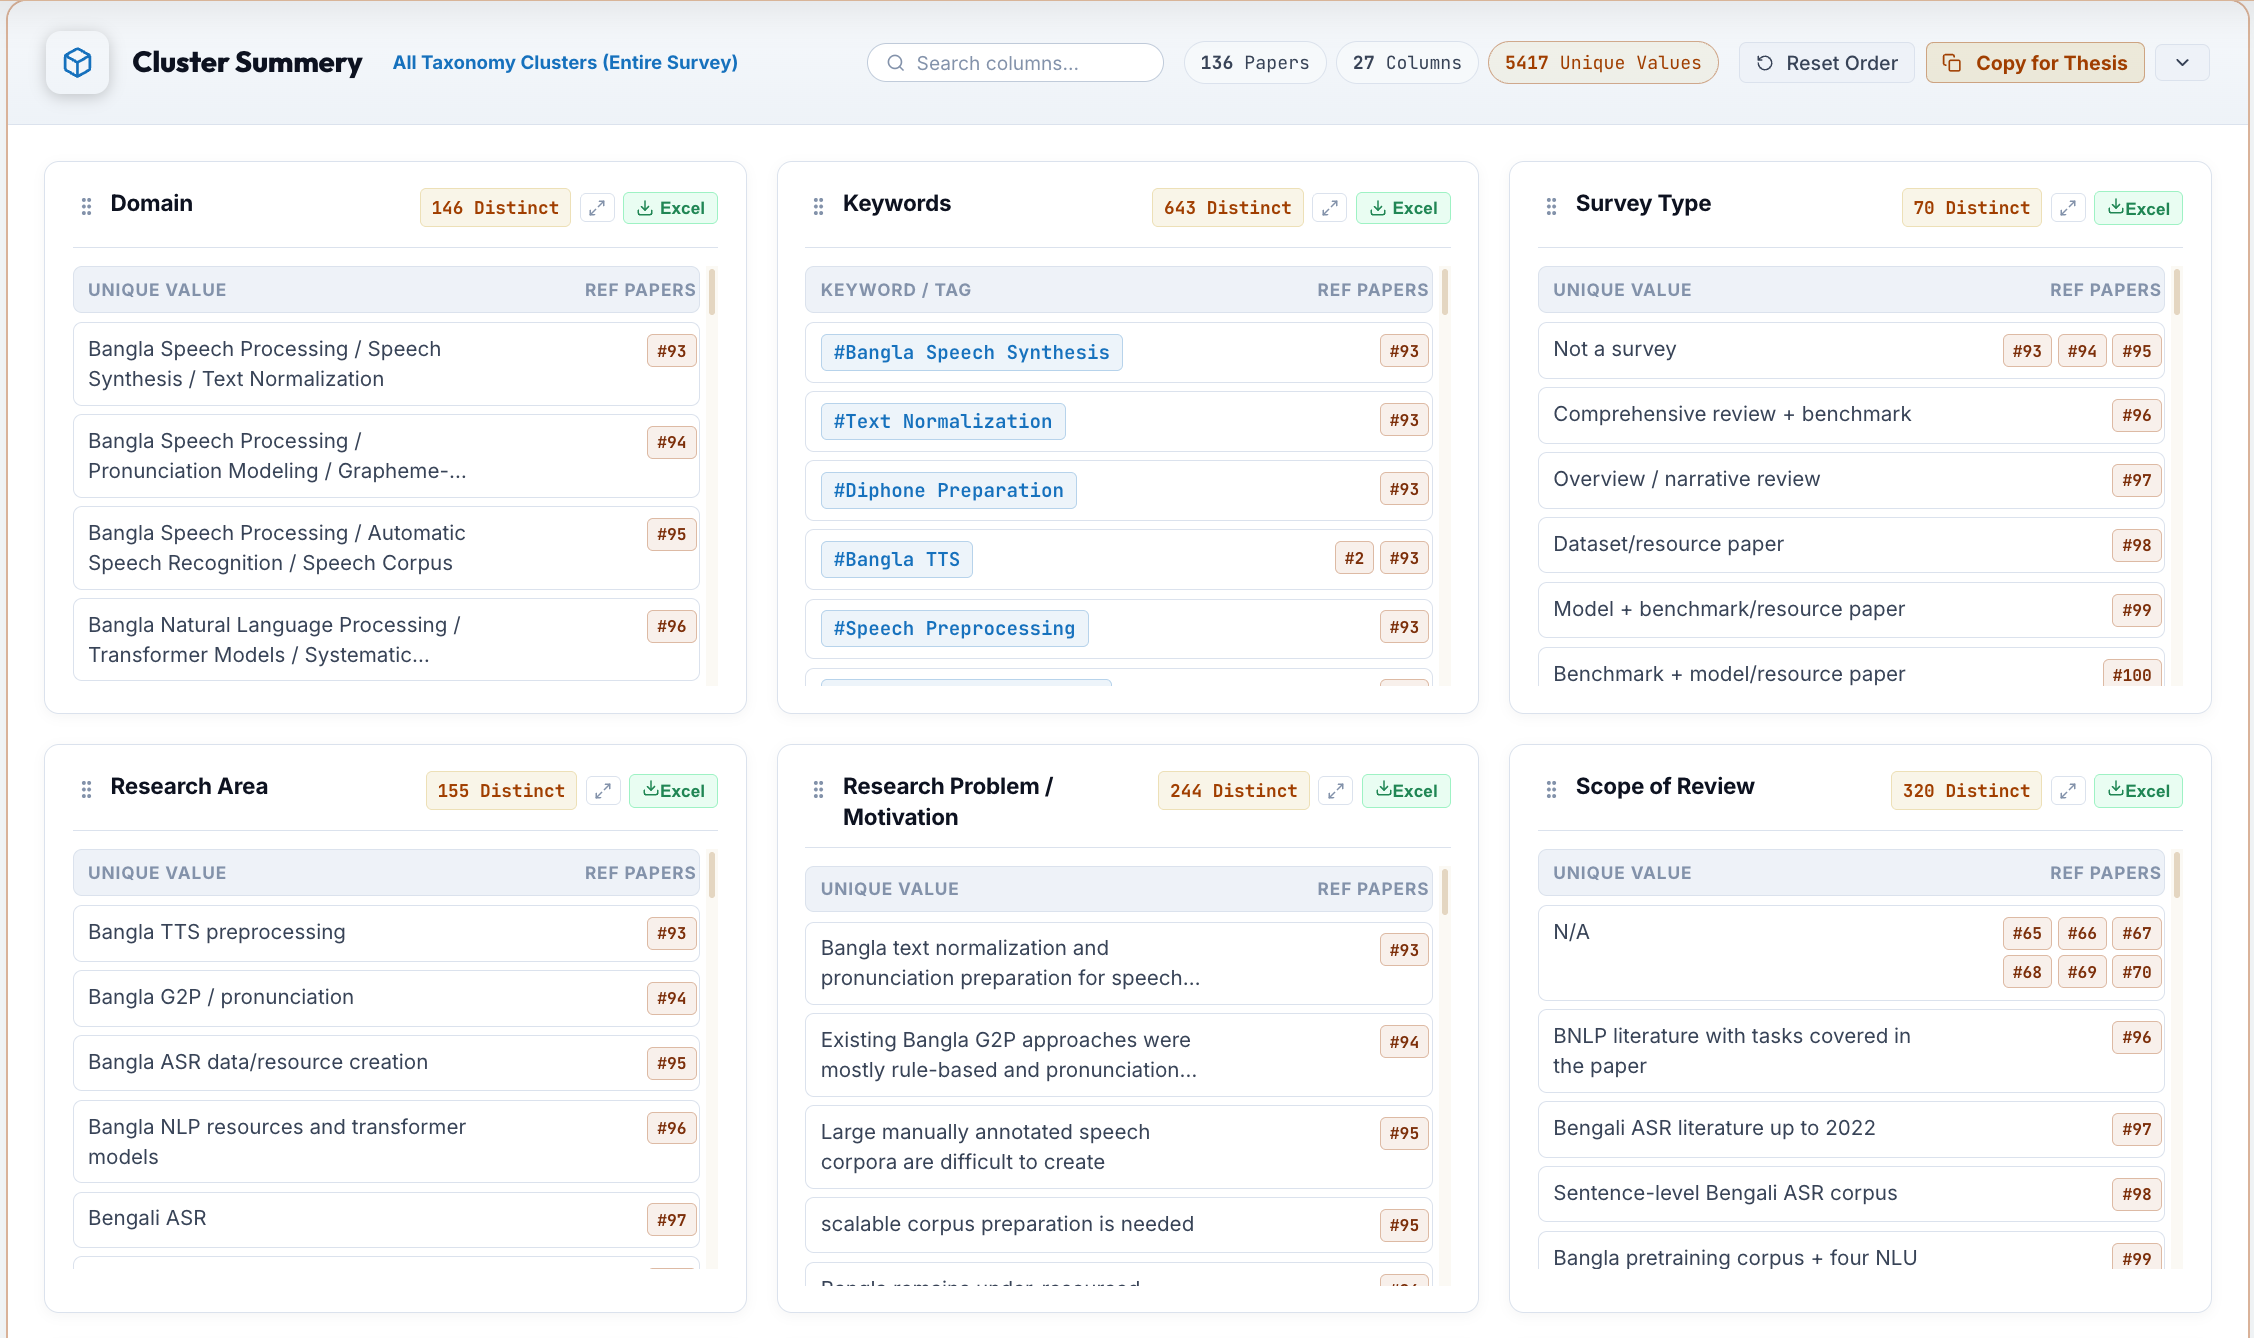
\includegraphics[width=13.6cm, height=3.80cm, keepaspectratio]{figures/ui_08_cluster_summary.png}%
}
\par\vspace{0.18cm}
\begin{columns}[T]
  \begin{column}{0.48\textwidth}
    \infoCard{6.8cm}{SubText}{TAXONOMY DISCOVERY}{Algorithmic Research Grouping}{%
      Automated thematic clustering categorizing ingested literature into distinct methodological paradigms, architectures, and focus domains.
    }
  \end{column}

  \begin{column}{0.48\textwidth}
    \infoCard{6.8cm}{SubText}{SYNTHESIS ANALYTICS}{Comparative Paradigm Distributions}{%
      Visual analytics displaying literature density, benchmark trends, and research frequency across surveyed publications.
    }
  \end{column}
\end{columns}
\end{frame}

% ==============================================================================
% SLIDE 27: UI: Benchmark Sample Analysis & Cluster Details
% ==============================================================================
\begin{frame}{UI: Benchmark Sample \& Cluster Details}
\vspace{-0.20cm}
\centering
\fboxrule=0.5pt\fboxsep=0pt\fcolorbox{black!15}{white}{%
  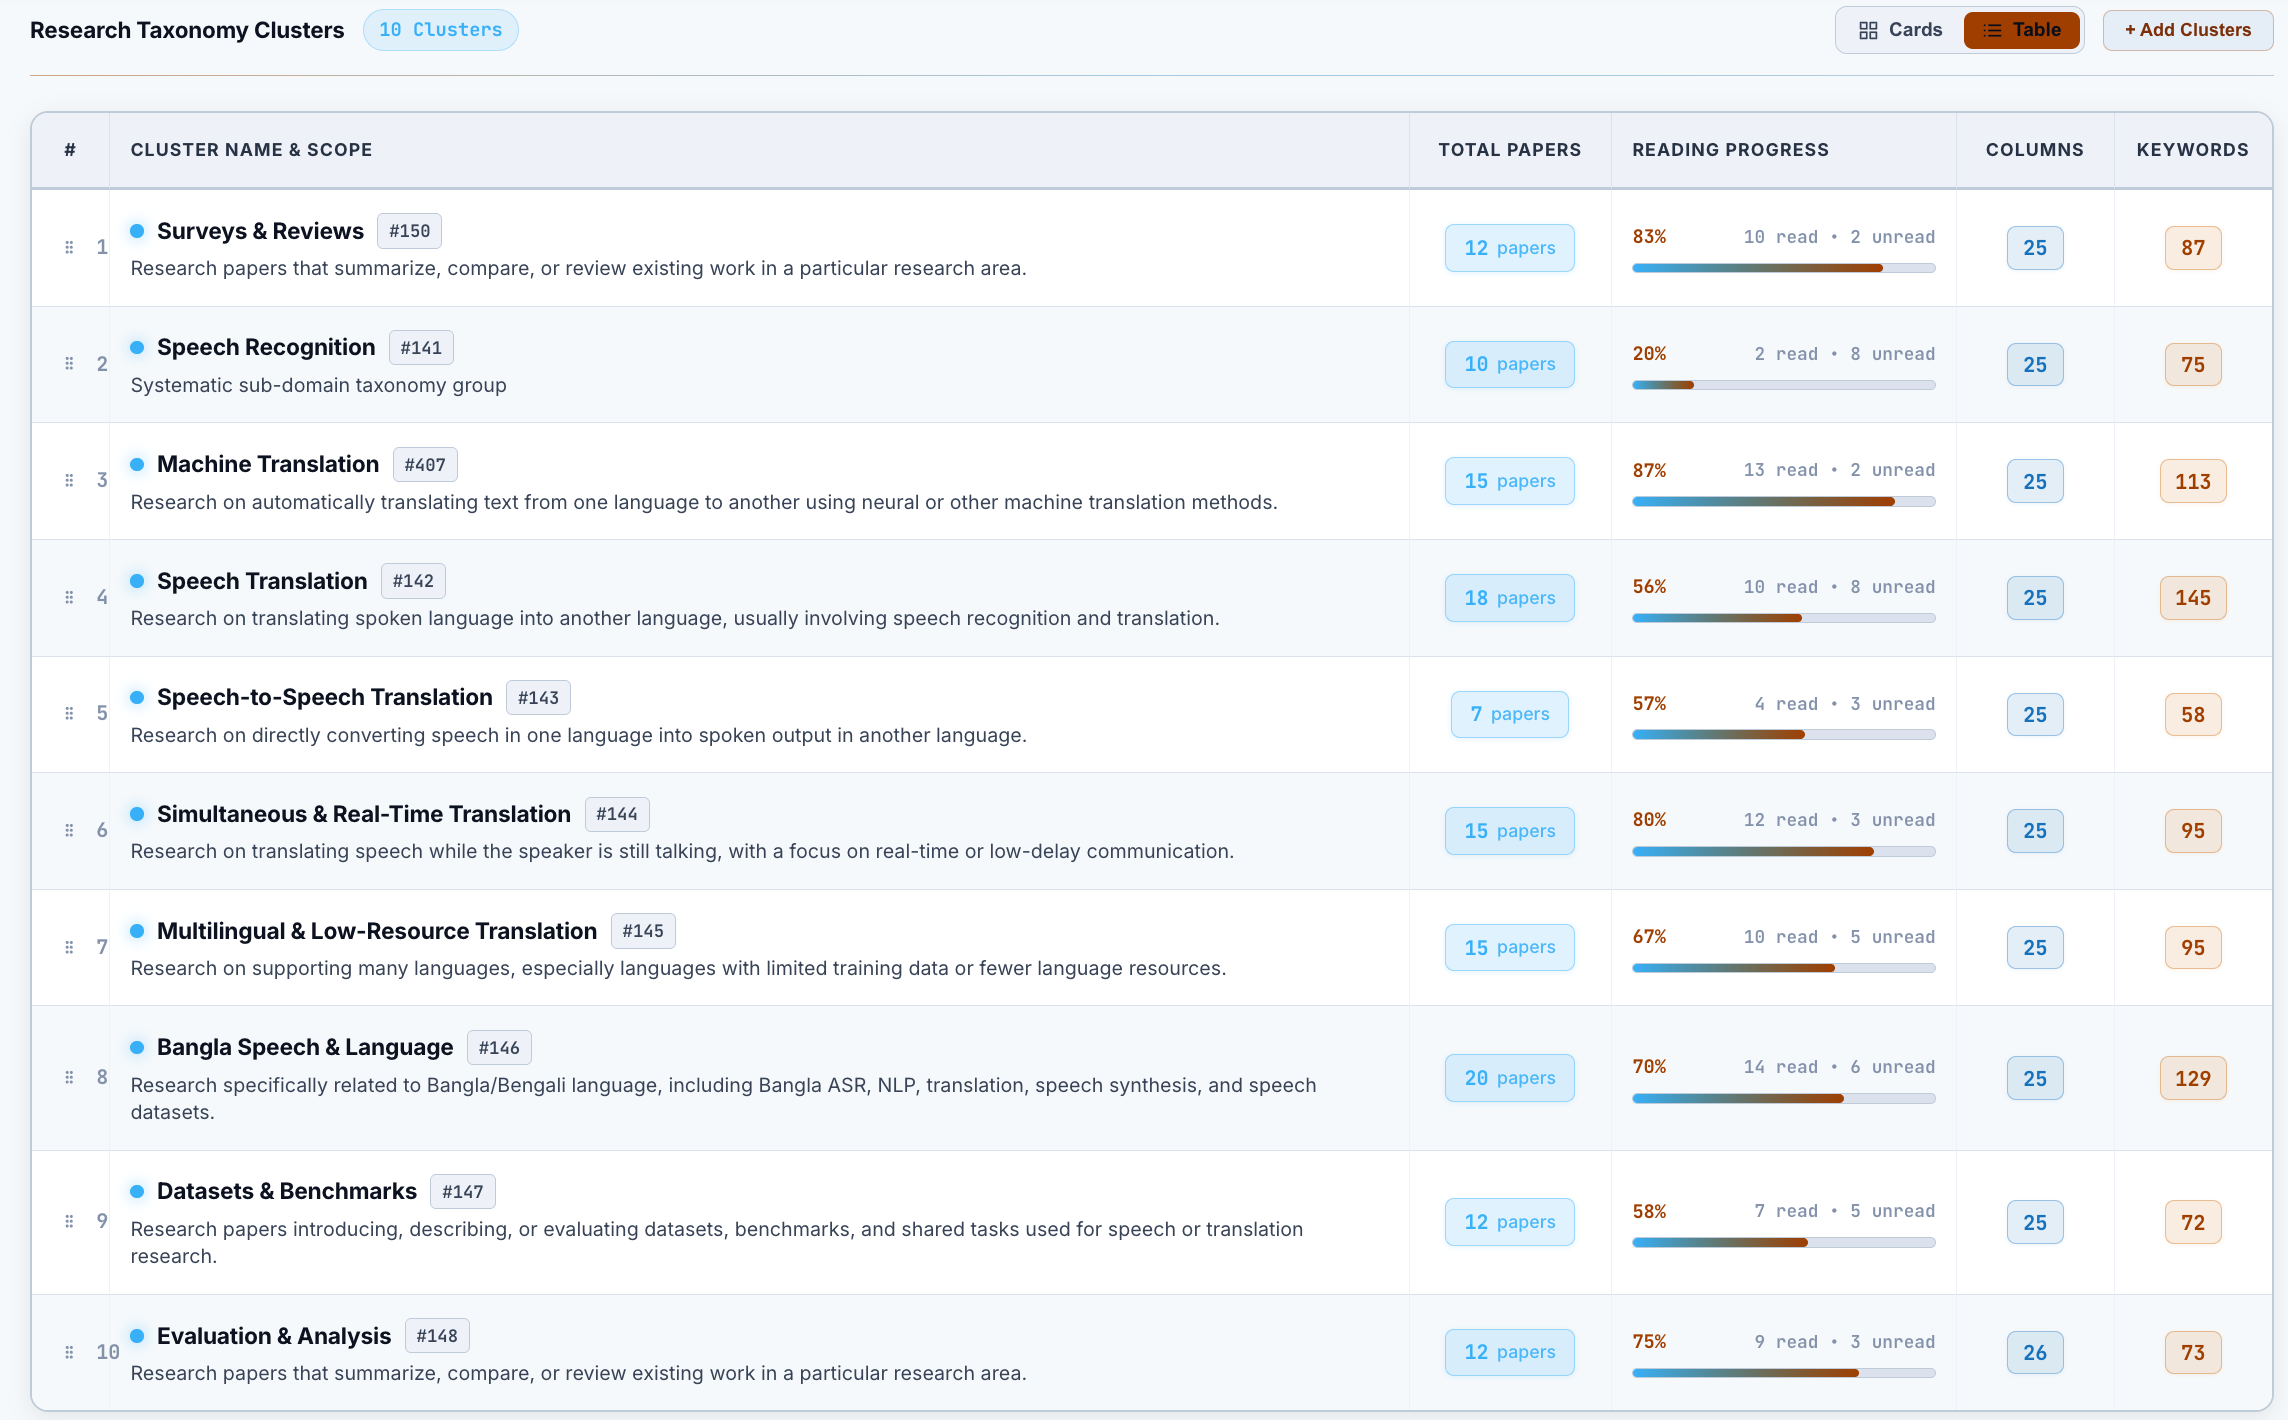
\includegraphics[width=13.6cm, height=3.80cm, keepaspectratio]{figures/ui_09_cluster_sample.png}%
}
\par\vspace{0.18cm}
\begin{columns}[T]
  \begin{column}{0.48\textwidth}
    \infoCard{6.8cm}{SubText}{GRANULAR DRILLDOWN}{Benchmark Sample Breakdown}{%
      Deep-dive inspection panel displaying constituent papers within a cluster, comparing evaluation metrics and algorithmic models.
    }
  \end{column}

  \begin{column}{0.48\textwidth}
    \infoCard{6.8cm}{SubText}{RESEARCH GAP IDENTIFICATION}{Cross-Methodology Discrepancies}{%
      Reveals performance discrepancies, benchmark dataset limitations, and unexplored research gaps across competitive methodologies.
    }
  \end{column}
\end{columns}
\end{frame}

% ==============================================================================
% SLIDE 28: Conclusion & Project Outlook
% ==============================================================================
\begin{frame}{Conclusion \& Project Outlook}
\vspace{-0.15cm}
\begin{columns}[T]
  \begin{column}{0.31\textwidth}
    {\fontsize{8.5pt}{10.5pt}\selectfont\bfseries\color{SubText} ACHIEVEMENTS}\par\vspace{3pt}
    {\fontsize{12pt}{14.5pt}\selectfont\bfseries\color{DarkText} Phases 1--3 Complete}\par\vspace{6pt}
    {\fontsize{9pt}{12pt}\selectfont\color{DarkText}
    \begin{itemize}\setlength{\itemsep}{4pt}
      \item End-to-end working system.
      \item Dual-pane PDF reviewer.
      \item Coordinate BBox anchoring.
      \item Live master matrix grid.
      \item Native LaTeX export.
    \end{itemize}}
  \end{column}

  \begin{column}{0.31\textwidth}
    {\fontsize{8.5pt}{10.5pt}\selectfont\bfseries\color{SubText} STATUS}\par\vspace{3pt}
    {\fontsize{12pt}{14.5pt}\selectfont\bfseries\color{DarkText} Current Milestone (M6)}\par\vspace{6pt}
    {\fontsize{9pt}{12pt}\selectfont\color{DarkText}
    \begin{itemize}\setlength{\itemsep}{4pt}
      \item 55\% roadmap executed.
      \item Zero major blockers.
      \item High UX performance.
      \item Proven architectural scale.
      \item On track for M12 defense.
    \end{itemize}}
  \end{column}

  \begin{column}{0.31\textwidth}
    {\fontsize{8.5pt}{10.5pt}\selectfont\bfseries\color{SubText} NEXT STEPS}\par\vspace{3pt}
    {\fontsize{12pt}{14.5pt}\selectfont\bfseries\color{DarkText} Months 7 to 12 Focus}\par\vspace{6pt}
    {\fontsize{9pt}{12pt}\selectfont\color{DarkText}
    \begin{itemize}\setlength{\itemsep}{4pt}
      \item Collaborative PRISMA voting.
      \item Cohen's Kappa score engine.
      \item Supervisor conflict resolver.
      \item SUS usability evaluation.
      \item Final thesis dissertation.
    \end{itemize}}
  \end{column}
\end{columns}
\end{frame}

\end{document}
